% Results overview
The results section is divided in three test cases: the Ringleb flow, the inviscid cylinder and the isentropic inviscid vortex. The former is intended to validate the high-order solver capabilities implemented in the present work and the others are used as comparative test cases between the single and overset mesh results. An important notation is used throughout the results section to notify the solver accuracy and mesh orders. For instance, a P2Q2 test considers a 2nd-order reconstruction of cell properties - a parabola, thus the P2 - which yields a 3rd-order accurate Spectral Difference method, with a 2nd-order construction of the quadrilateral mesh, which means that cell edges are parabolas, and thus the denomination Q2. 
% which tests, where are they from (HiOCFD Workshop) 
%For the oversets a comparisom between single and overset grids are made. Residue and 
%For high-order solver implementation,  accuracy tests.

\section{Ringleb Flow}
%
The Ringleb flow is a common candidate to state the level of accuracy in high-order solvers due to its analytical solution for the Euler Equations derived from a hodograph transformation \cite{Shapiro1953}. Another interesting property of the Ringleb flow is that the transition from supersonic to subsonic region does not generate a shock, then no limiter is needed. The analytical solution is used as initial condition and only depends on three parameters: the velocity magnitude $q$ and the stream function interval given by $[k_{min}, k_{max}]$. The stream function interval defines the stream lines for the inner wall, $k_{max}$, and outer wall, $k_{min}$. The mesh for the Ringleb flow is defined through the hodograph transformation of the Euler Equations and therefore a relation from the fluid properties to the $x, y$ coordinates is established. The velocity magnitude $q$ varies between $q_0$ and $k$, for each $k$ in the interval $k_{min} \leq k \leq k_{max}$. For each velocity magnitude $q$, the speed of sound $a$, density $\rho$, pressure $p$ and quantity $M$ can be defined by
%
\begin{equation}
    \label{eq_ringleb_analytical_1}
	a = \sqrt{1 - \frac{\gamma -1}{2}q^2}; \rho = a^{\frac{2}{\gamma -1}}; p = \frac{1}{\gamma}a^{\left(\frac{2\gamma}{\gamma - 1}\right)}
\end{equation}
% 
\begin{equation}
    \label{eq_ringleb_analytical_2}
	 M = \frac{1}{a} + \frac{1}{3a^3} + \frac{1}{5a^5} - \frac{1}{2} log\frac{1+a}{1-a}.
\end{equation}
%
where $\gamma$ is 1.4 for the air. 
For each pair $(q, k)$, the mesh coordinate $x, y$ can be determined by
%
\begin{equation}
    \label{eq_ringleb_mesh_x}
	x(q, k) = \frac{1}{2p}\left(\frac{2}{k^2}-\frac{1}{q^2}\right)-\frac{M}{2}
\end{equation}
%
\begin{equation}
    \label{eq_ringleb_mesh_y}
	y(q, k) = \pm \frac{1}{k\rho q} \sqrt{1 - \left(\frac{q}{k}\right)^2}
\end{equation}
%
The results obtained in this test case considered $q_0=0.5$, $k_{min}=0.7$ and $k_{max}=1.5$. The boundary conditions are imposed with a subsonic inlet at the top, a subsonic outlet at the bottom and the exact analytical solution at the inner (left) and outer (right) walls as illustrated in Fig.\ \ref{fig:ringleb_bc}. The mesh is gathered from the 4th High-Order CFD Workshop \cite{4thHOW} containing 12 fourth-order cells (Q4). As it can be seen in the Ringleb flow boundary conditions illustrated in Fig.\ \ref{fig:ringleb_bc}, the inflow and outflow area are also curved and, therefore, the Q4 high-order mesh is chosen to represent it. The initial input mesh for this test case is illustrated in Fig.\ \ref{fig:ringleb_mesh_0} representing a Ringleb mesh with $q_0=0.5$, $k_{min}=0.7$ and $k_{max}=1.5$.
%
\begin{figure}[H]
	\centering
	 \subfigure[][]
	{
        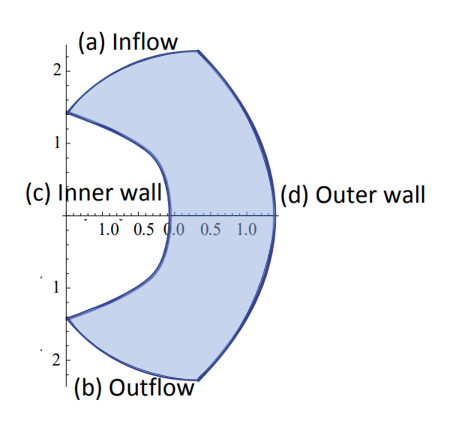
\includegraphics[height=8.0cm]{figs/results/ringleb/ringleb_boundary_condition.png}
		\label{fig:ringleb_bc}
    }
    \subfigure[][]
	{
        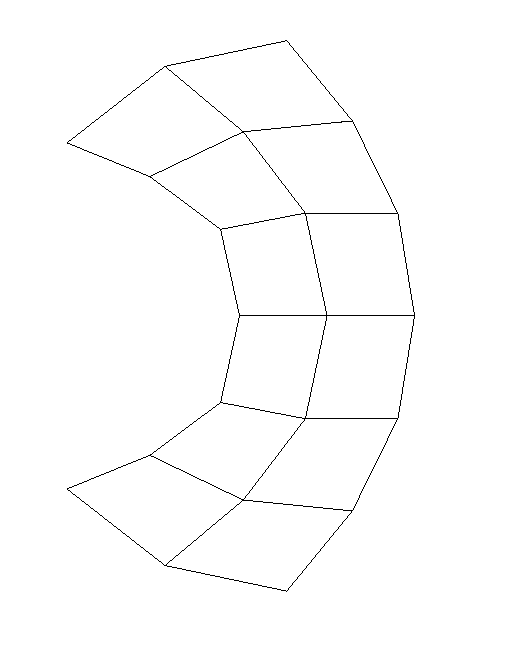
\includegraphics[height=8.0cm]{figs/results/ringleb/solution/ringleb_mesh_0.png}
		\label{fig:ringleb_mesh_0}
    }
    \caption{Ringleb flow boundary conditions (left) and initial mesh (right).}
    \label{fig:ringleb_boundary_condition}
\end{figure}
%
% Meshes (initial and high-order p meshes)
The Spectral Difference method is used with several polynomial orders ranging from $P=2$ up to $P=5$ and Fig.\ \ref{fig:ringleb_meshes} shows the correspondent pos-processing mesh and close-up views. The pos-processing mesh is generated through all the cells vertices, solution and flux points with no information lost. Additionally, since only the solution points own the final converged solution, in the pos-processing procedure, the solution is interpolated from the solution points to the flux-points and vertices where an average is applied to smooth the solution. In the close-up images from Fig.\ \ref{fig:ringleb_meshes}, one may compare the different degrees of freedom between the selected $P$ for the same 12 cell mesh used in the entire test.

\begin{figure}[H]
	\centering
    \subfigure[][P2Q4.]
	{
        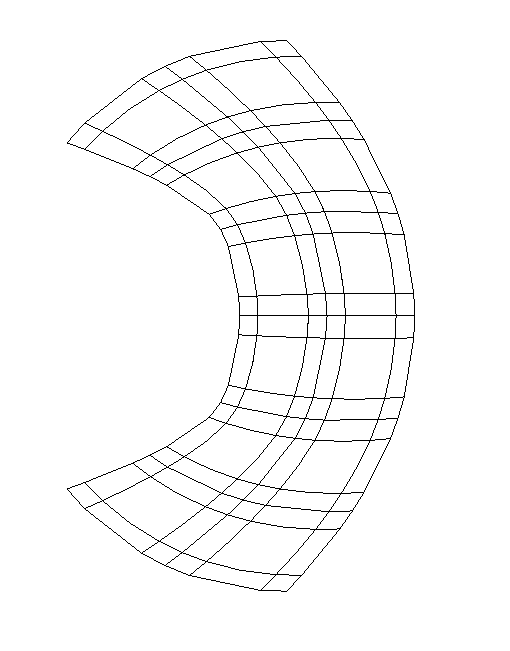
\includegraphics[height=4.0cm]{figs/results/ringleb/solution/ringleb_mesh_p_2.png}
		\label{fig:ringleb_mesh_2}
    }
    \subfigure[][P3Q4.]
	{
        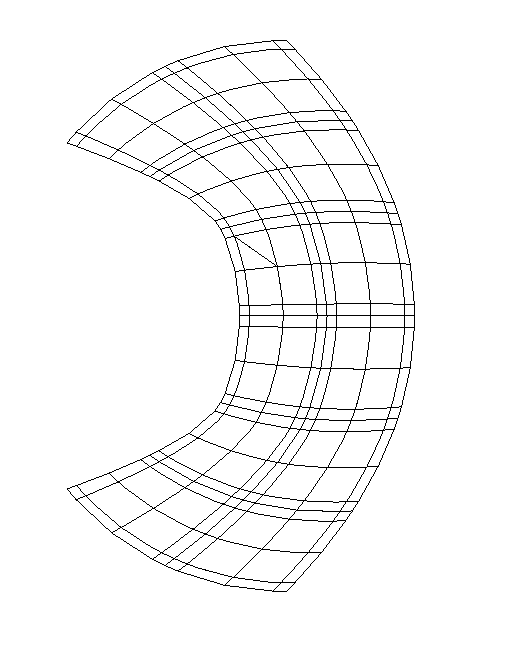
\includegraphics[height=4.0cm]{figs/results/ringleb/solution/ringleb_mesh_p_3.png}
		\label{fig:ringleb_mesh_3}
    }
    \subfigure[][P4Q4.]
	{
        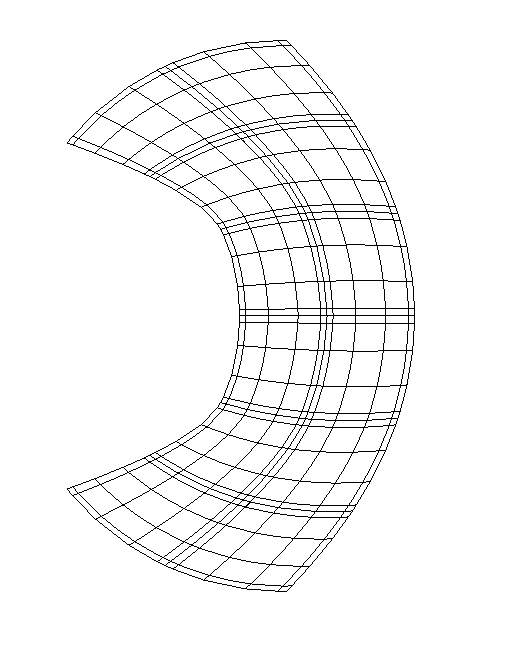
\includegraphics[height=4.0cm]{figs/results/ringleb/solution/ringleb_mesh_p_4.png}
		\label{fig:ringleb_mesh_4}
    }
    \subfigure[][P5Q4.]
	{
        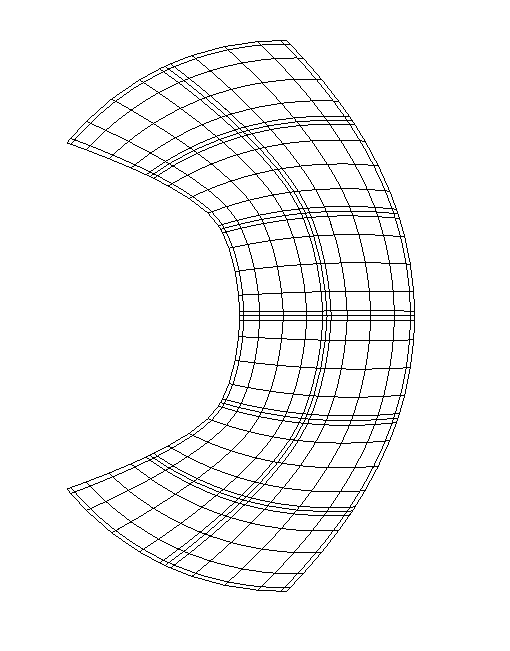
\includegraphics[height=4.0cm]{figs/results/ringleb/solution/ringleb_mesh_p_5.png}
		\label{fig:ringleb_mesh_5}
    }
     \subfigure[][P2Q4 close-up.]
	{
        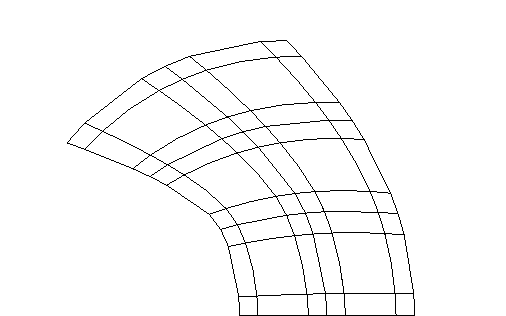
\includegraphics[height=4.0cm]{figs/results/ringleb/solution/ringleb_mesh_p_2_cp.png}
		\label{fig:ringleb_mesh_2_cp}
    }
    \subfigure[][P3Q4  close-up.]
	{
        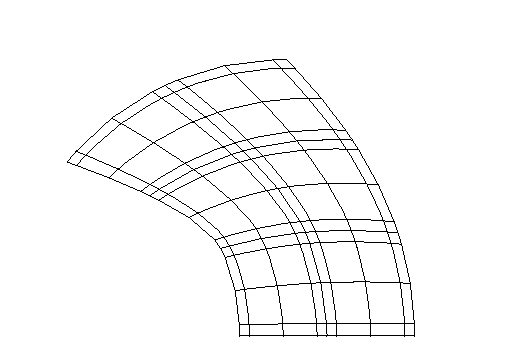
\includegraphics[height=4.0cm]{figs/results/ringleb/solution/ringleb_mesh_p_3_cp.png}
		\label{fig:ringleb_mesh_3_cp}
    }
    \subfigure[][P4Q4  close-up.]
	{
        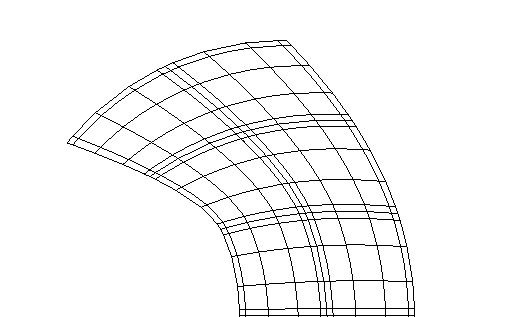
\includegraphics[height=4.0cm]{figs/results/ringleb/solution/ringleb_mesh_p_4_cp.png}
		\label{fig:ringleb_mesh_4_cp}
    }
    \subfigure[][P5Q4  close-up.]
	{
        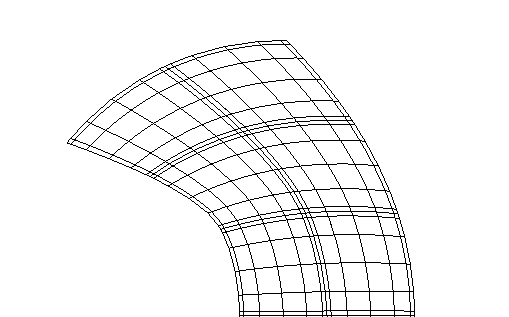
\includegraphics[height=4.0cm]{figs/results/ringleb/solution/ringleb_mesh_p_5_cp.png}
		\label{fig:ringleb_mesh_5_cp}
    }
    \caption{Meshes for the Ringleb flow test case for different P values.}
    \label{fig:ringleb_meshes}
\end{figure}

% how to gather the analytical solution
The analytical solution is determined by solving Eqs.\ \ref{eq_ringleb_mesh_x} and \ref{eq_ringleb_mesh_y} numerically  over $q$ with a Newton Raphson algorithm. The analytical values for the velocity components, $u$ and $v$, are defined by $u = \pm q cos(\theta)$ and $v = -q sin(\theta)$, where $\theta = asin \left(\frac{q}{k}\right)$. Additionally, the $u$ velocity component direction changes depending on the $y$ coordinate sign. Figure\ \ref{fig:ringleb_analytical_solution} presents the analytical Mach number solution considering $q_0=0.5$, $k_{min}=0.7$ and $k_{max}=1.5$ with a colormap ranging from $0.5$ to $2.0$. The analytical Mach number solution shows a symmetrical solution over the x axis with the presence of supersonic regions, despite no shock is formed and then a smooth solution is expected.

% Analytical Solution
\begin{figure}[H]
	\centering
	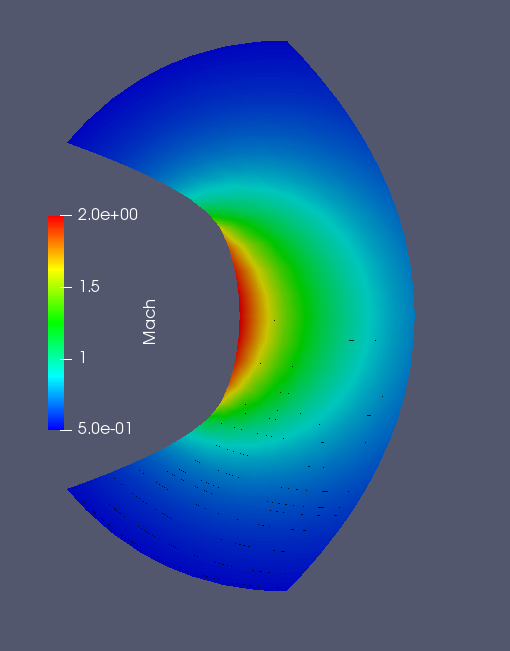
\includegraphics[height=8.0cm]{figs/results/ringleb/solution/ringleb_initial_solution.png}
    \caption{Analytical Ringleb flow solution: Mach number contours.}
    \label{fig:ringleb_analytical_solution}
\end{figure}

% describe the residue for each p
The simulation results for the L2-norm of the density residue are shown in Fig.\ \ref{fig:ringleb_residue} for different orders of the Spectral Difference method. The L2-norm is calculated over all solution points considering the entire residue vector norm, {\em i.e.}, the residue of all conservative properties. The time integration method is a SSP Runge-Kutta scheme of 3rd order and 3 stages. The time step is fixed for each simulation and it is given by Eq.\ \ref{eq_ssp_rk_time_step}. Consequently, for higher values of $P$, the time step decreases. As it can be seen in Fig.\ \ref{fig:ringleb_residue}, the slope of the lines representing the residue order of magnitude rate of change is almost constant for each $P$ value. Additionally, for all test cases, {\em i.e.}, for all $P$ values, the solution has converged to machine zero error.

% Residue history for different p
\begin{figure}[H]
	\centering
	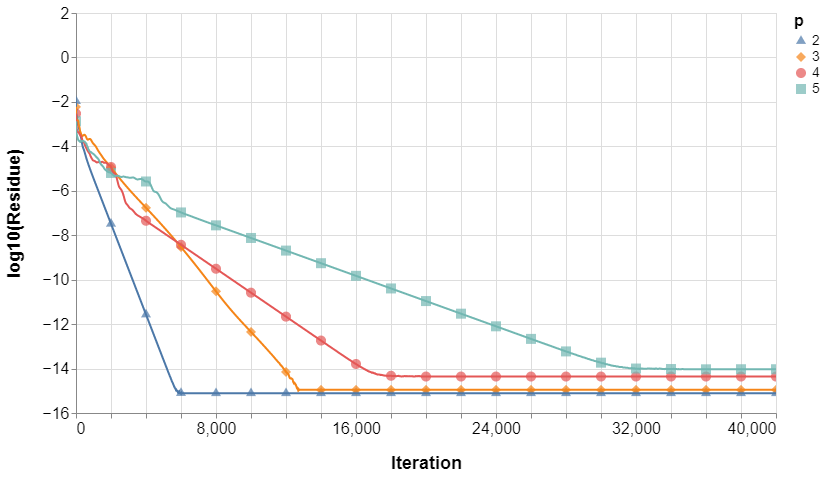
\includegraphics[height=9.0cm]{figs/results/ringleb/ringleb_residue_by_p.png}
    \caption{L2-norm of the density residue for the Ringleb flow for different values of P for the same mesh (Q4).}
    \label{fig:ringleb_residue}
\end{figure}

% mach contours, comment about the symmetry when p >= q
The converged Mach number solutions for different $P$ values are presented in Fig.\ \ref{fig:ringleb_mach} containing the field colormap ranging from $0.5$ to $2.0$ and contours with $0.1$ step value. For 2nd and 3rd-order of solution polynomial reconstruction, {\em i.e.},  $P=2$ and $P=3$, despite the fact that convergence to the machine error level has been reached, the Mach number contours in Figs.\ \ref{fig:ringleb_mach_2} and \ref{fig:ringleb_mach_3} presented asymmetries with regard to the x-axis and spikes in the colormap close to the outlet, where the velocity magnitude showed higher values than expected according to the provided analytical solution in Fig.\ \ref{fig:ringleb_analytical_solution}. On the other hand, when the spatial discretization method order is greater or equal to the presented mesh order, the asymmetries are eliminated. As it can be seen in Figs.\ \ref{fig:ringleb_mach_4} and \ref{fig:ringleb_mach_5}, respectively, for $P=4$ and $P=5$ with the 4th order mesh, the numerical Mach number solution captures the shockless supersonic region which can be compared to the analytical solution.
% future calculate the entropy error
% Mach contours
\begin{figure}[H]
	\centering
    \subfigure[][P2Q4.]
	{
        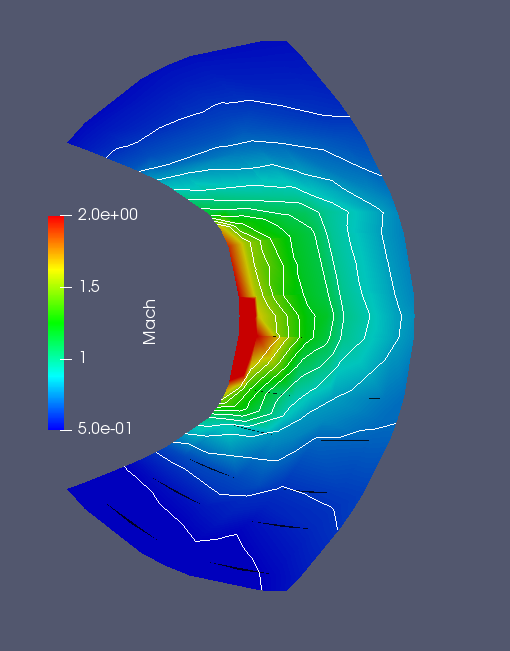
\includegraphics[height=8.5cm]{figs/results/ringleb/solution/ringleb_sol_mach_p2.png}
		\label{fig:ringleb_mach_2}
    }
    \subfigure[][P3Q4.]
	{
        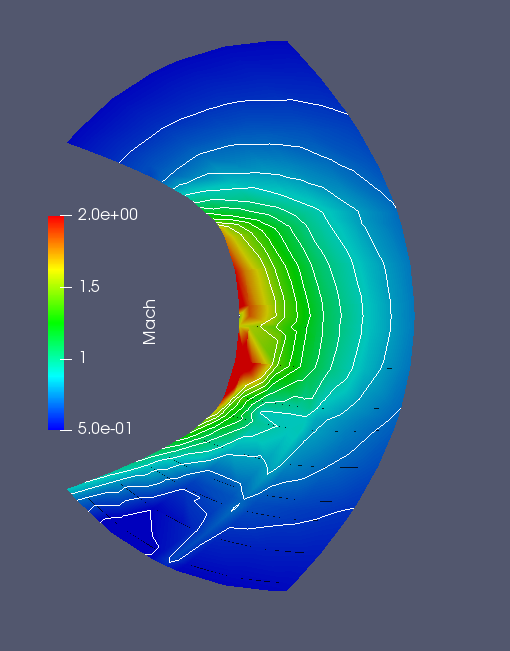
\includegraphics[height=8.5cm]{figs/results/ringleb/solution/ringleb_sol_mach_p3.png}
		\label{fig:ringleb_mach_3}
    }
    \subfigure[][P4Q4.]
	{
        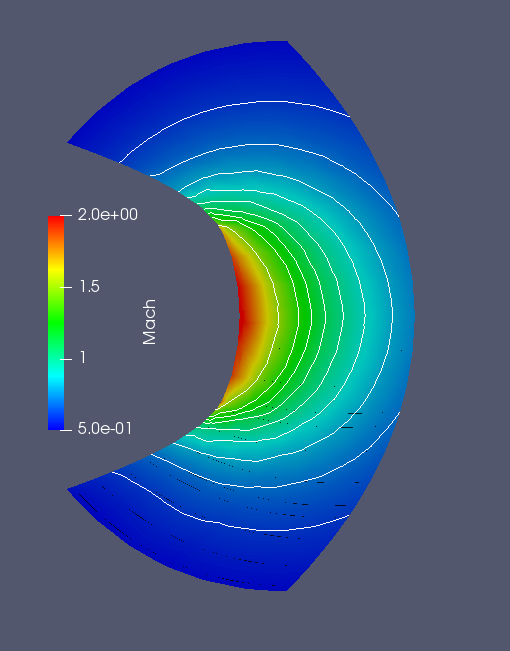
\includegraphics[height=8.5cm]{figs/results/ringleb/solution/ringleb_sol_mach_p4.png}
		\label{fig:ringleb_mach_4}
    }
    \subfigure[][P5Q4.]
	{
        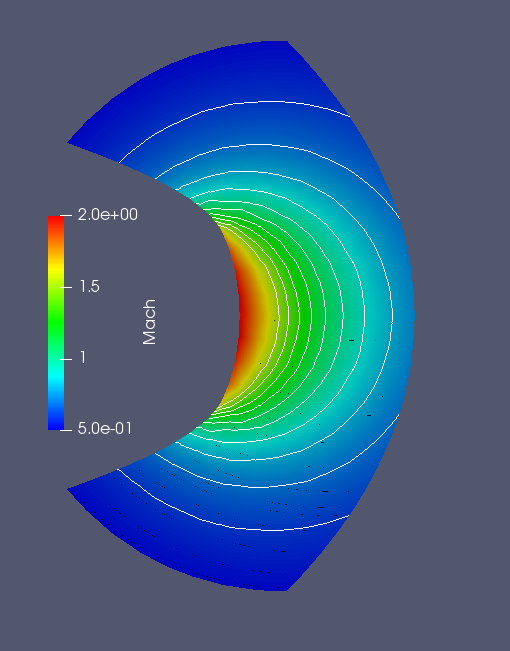
\includegraphics[height=8.5cm]{figs/results/ringleb/solution/ringleb_sol_mach_p5.png}
		\label{fig:ringleb_mach_5}
    }
    \caption{Converged numerical Mach number contour solution for the Ringleb flow test case for different P values.}
    \label{fig:ringleb_mach}
\end{figure}

\section{Inviscid Cylinder}

% Problem setup
A subsonic inviscid flow over a cylinder is considered to compare the single and overset mesh results. The simulation is setup with a free-stream Mach number of 0.2 in order to observe a double symmetry at the horizontal and vertical axis for the Mach number field solution when solving the Euler equations. The mesh domain is defined with a 100-cylinder radius with the overall initial condition of $Mach=0.2$, $\rho=1$ and $p=\frac{1}{\gamma}$ assuming $\gamma=1.4$ for the air. Figure\ \ref{fig:cylinder_boundary_conditions} illustrates the sketch for the boundary condition setup for the single mesh and overset mesh cases.

Initially, the imposed boundary conditions considered a subsonic or supersonic inlet - depending on the normal face velocity - forcing the free-stream Mach at the entrance, an outlet at the exit forcing $p=\frac{1}{\gamma}$ for subsonic and internal solution extrapolation for supersonic, and a slip wall condition at the cylinder. The initial solution in the fluid domain is imposed as the free stream conservative properties. However, despite the fact that the outer boundary is defined at a 100-cylinder radius away from the body, a residue wave stayed in the domain initiated at the first step due to the abrupt initial solution imposed around the cylinder, where the normal velocity component is zero and the fluid domain properties are the free stream values. Therefore, the farfield boundary conditions had to be modified in order to impose a non-reflective farfield and, hence, overcome the difficulty described, as sketched in Fig.\ \ref{fig:cylinder_boundary_conditions}. For the overset case, the cells around the external boundary of the near-body mesh are marked as an overset region during the mesh generation. These overset flags are used in the receptor-donor connectivity procedure to establish how the data is interpolated from one mesh to the other at each time step.

% add boundary condition image
 \begin{figure}[H]
	\centering
	 \subfigure[][Single mesh boundary conditions.]
	{
        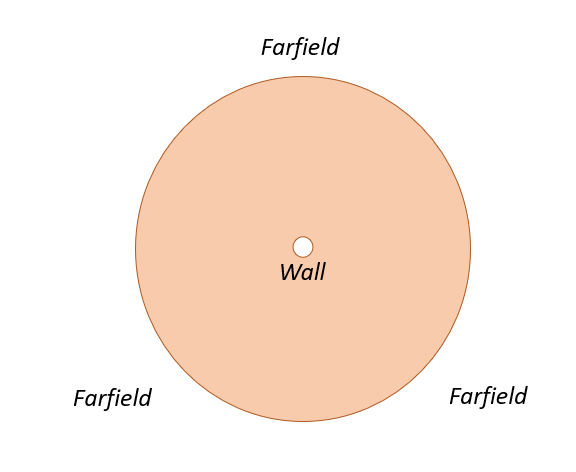
\includegraphics[height=6.0cm]{figs/results/cylinder/cylinder_bc_single.PNG}
		\label{fig:cylinder_bc}
    }
    \subfigure[][Overset meshes boundary conditions.]
	{
        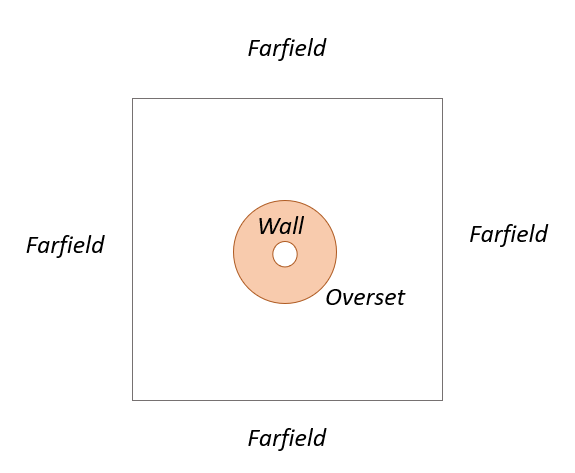
\includegraphics[height=6.0cm]{figs/results/cylinder/cylinder_bc_overset.PNG}
		\label{fig:cylinder_mesh_0}
    }
    \caption{Inviscid cylinder boundary conditions sketch for single mesh (left) and overset mesh (right) cases.}
    \label{fig:cylinder_boundary_conditions}
\end{figure}
%

% Meshes (single and overset)
The meshes generated for the present tests considered a mesh with $20 \times 32$ cells for the single mesh case, two background meshes, a $32 \times 32$ and a $24 \times 24$ cells, and a near-body mesh with $20 \times 20$ cells as illustrated in Fig.\ \ref{fig:sin_cyl_mesh}.  The $24 \times 24$ background mesh illustrated in Fig.\ \ref{fig:overset_msh_24} has a refinement at the central horizontal and vertical lines that crosses the cylinder center. The reason for this refinement is due to difficulties in edge cases for the cells at the overset region. Occasionally, a fringe cell flux point, that requires interpolated data, may not be embedded by a donor cell. Moreover, since its neighbor cell is deactivated, {\em i.e.}, it is a hole cell, no flux is defined in this interface during the simulation making the solution to diverge. Hence, the length scale around the overset region between the background and near-body mesh needs to be similar so that the receptor-donor relationship can be fully established altogether with the existence of the fringe circuit which limits the BFS hole propagation.
%
\begin{figure}[H]
	\centering
	% 20x32 single mesh
	\subfigure[][$20 \times 32$ - single mesh view.]
	{
        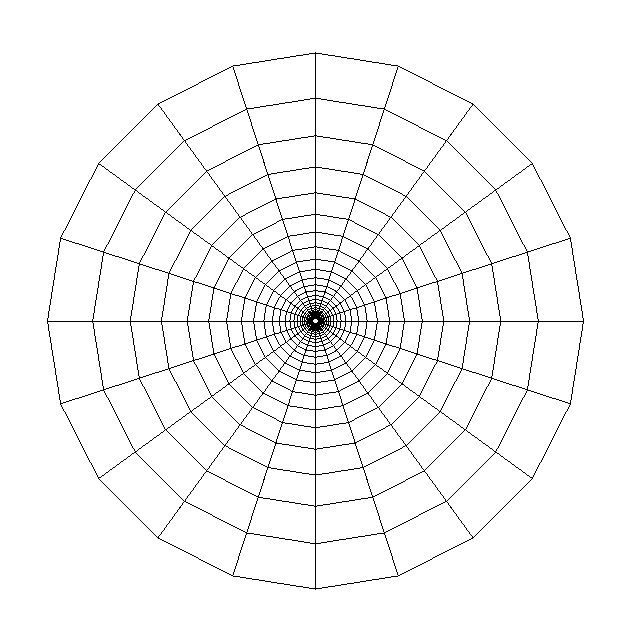
\includegraphics[height=5.5cm]{figs/results/cylinder/solution/mesh_single.png}
		\label{fig:single_msh}
    }
    \hfill
    \subfigure[][$20 \times 32$ - single mesh close-up view.]
    {
		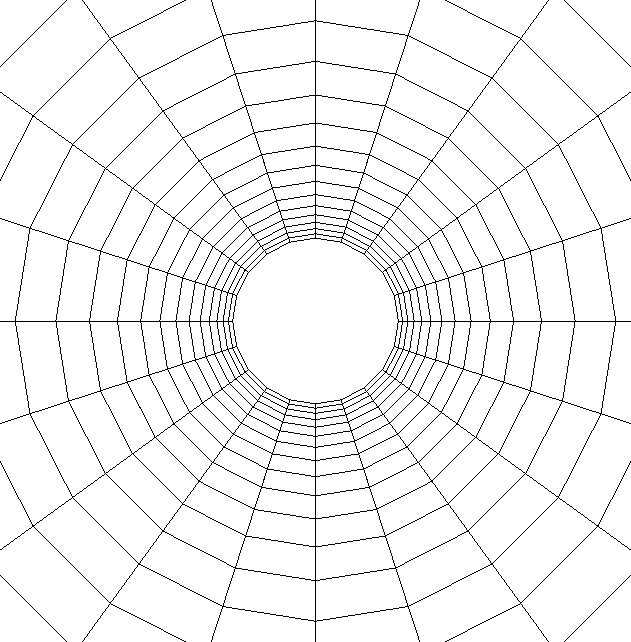
\includegraphics[height=5.5cm]{figs/results/cylinder/solution/mesh_single_closeup.png}
		\label{fig:single_msh_cp}
    }
    \hfill
    % 32x32 background and 20x20 near-body overset mesh 
    \subfigure[][$32 \times 32$ background and $20 \times 20$ near-body mesh view.]
	{
        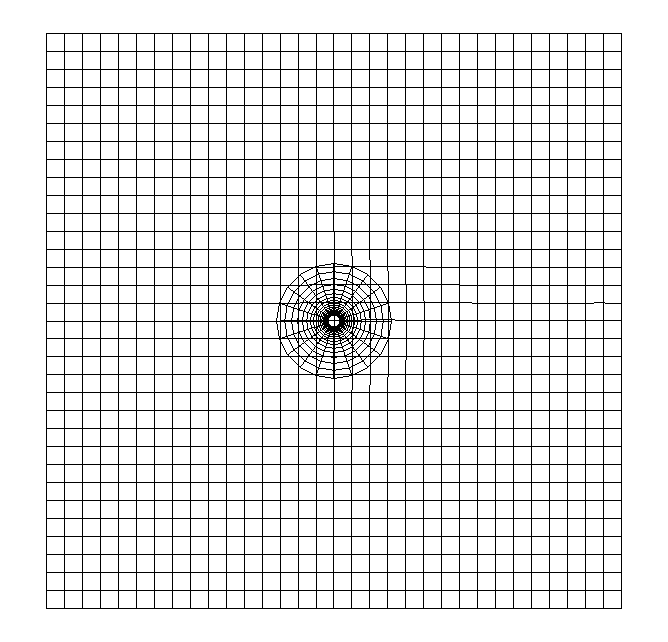
\includegraphics[height=5.5cm]{figs/results/cylinder/solution/mesh_overset_lo.png}
		\label{fig:overset_msh_32}
    }
    \hfill
    \subfigure[][$32 \times 32$ background and $20 \times 20$ near-body mesh close-up view.]
    {
		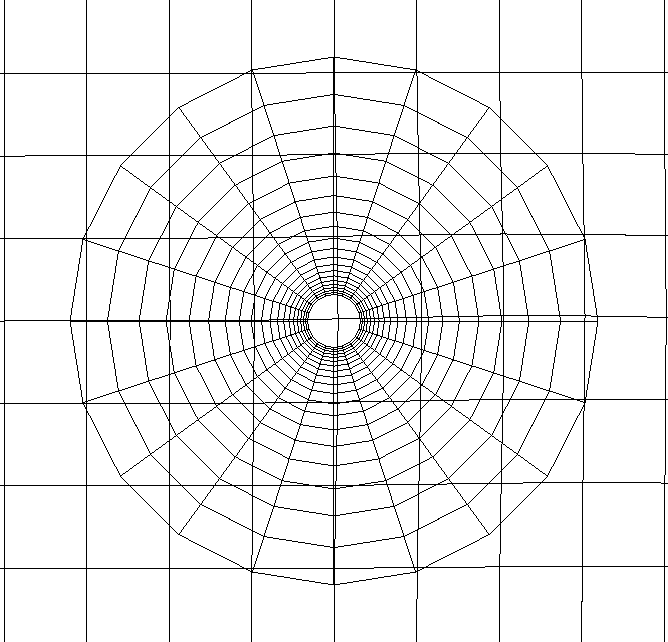
\includegraphics[height=5.5cm]{figs/results/cylinder/solution/mesh_overset_lo_closeup.png}
		\label{fig:overset_msh_32_cp}
    }
    \hfill
    % 24x24 background and 20x20 near-body overset mesh 
     \subfigure[][$24 \times 24$ background and $20 \times 20$ near-body mesh view.]
	{
        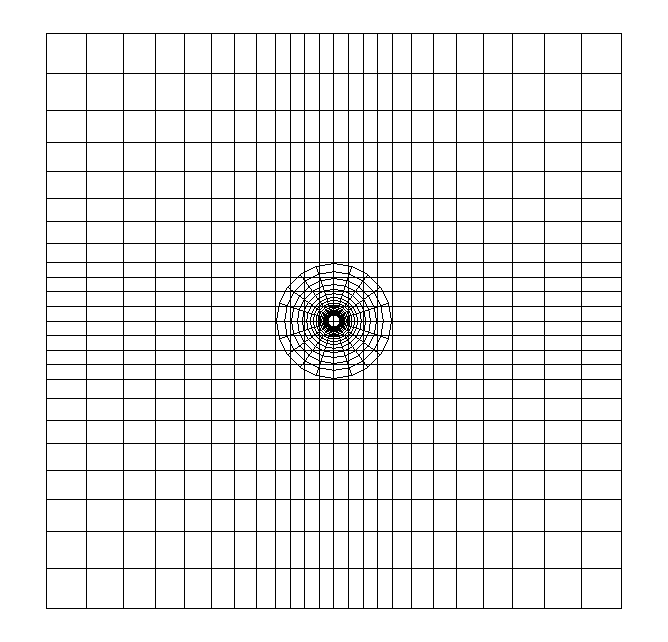
\includegraphics[height=5.5cm]{figs/results/cylinder/solution/mesh_overset_ho.png}
		\label{fig:overset_msh_24}
    }
    \hfill
    \subfigure[][$24 \times 24$ background and $20 \times 20$ near-body mesh close-up view.]
    {
		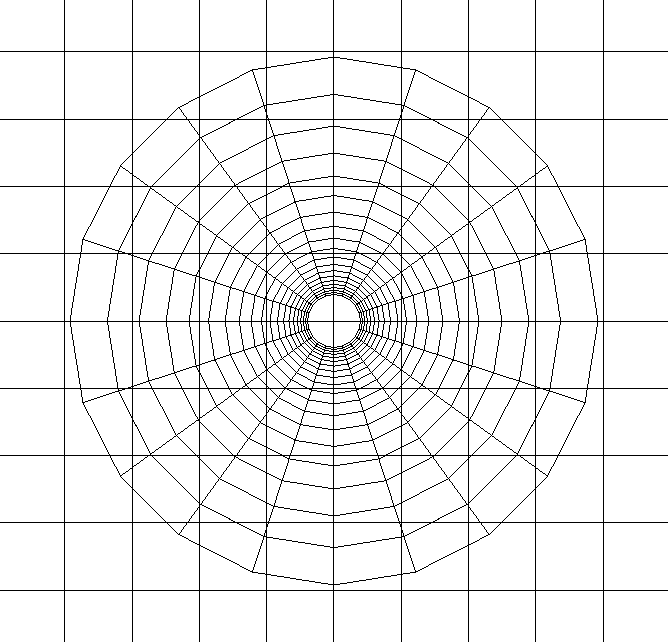
\includegraphics[height=5.5cm]{figs/results/cylinder/solution/mesh_overset_ho_closeup.png}
		\label{fig:overset_msh_24_cp}
    }
    \caption{Cylinder single and overset meshes with 1:100 cylinder radius ratio.}
    \label{fig:sin_cyl_mesh}
\end{figure}

Two different scenarios are tested over the inviscid cylinder test case: a low-order case with P2Q1 and a high-order case with P5Q4 resolution. Figure\ \ref{fig:msh_cylinder_sd} shows the close-up views of the Spectral Difference meshes around the cylinder walls obtained from the aforementioned grids. The grid length scale around the cylinder is imposed to be similar between the single and near-body meshes so that the number of degrees of freedom can be comparable. Although, the effect of curvature is not visually noticeable for the P5Q4 linear visualization of the grid points in Figs.\ \ref{fig:sin_msh_cyl_ho} and \ref{fig:ovs_msh_cyl_ho}, the position of the flux-points and the entire standard space projection is affected through the high-order Jacobian representation over a high-order cell.

% SD Meshes
\begin{figure}[H]
	\centering
    \subfigure[][Low-order cylinder single mesh, P2Q1.]
    {
		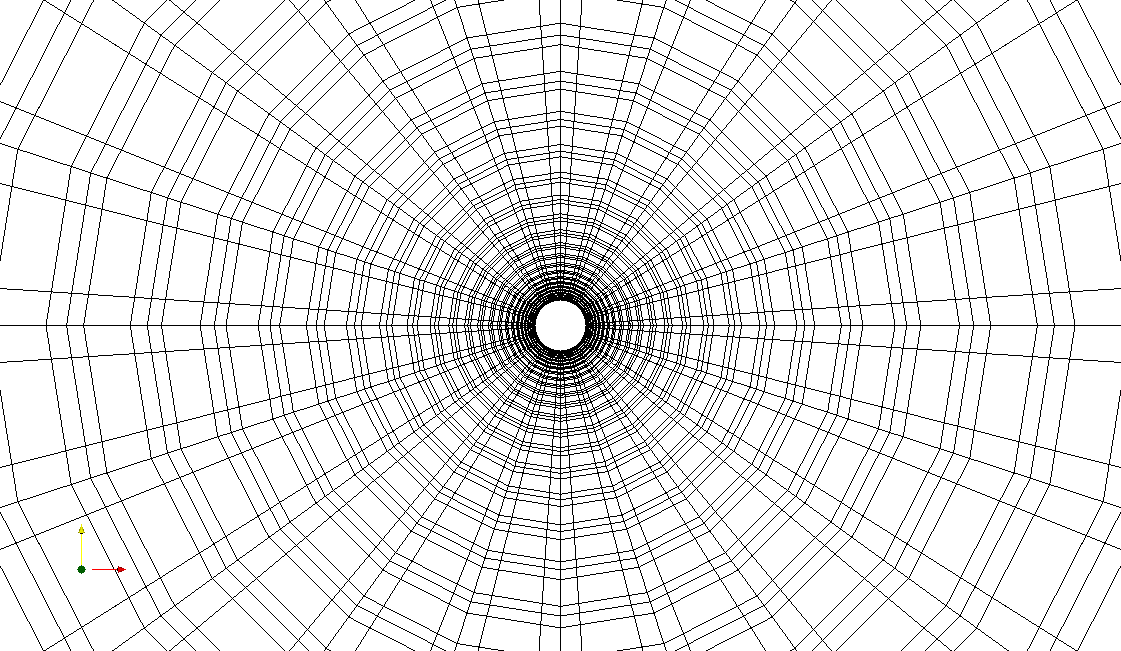
\includegraphics[height=4.3cm]{figs/results/cylinder_overset/lo_cylinder_mesh.png}
		\label{fig:sin_msh_cyl_lo}
    }
    \subfigure[][Low-order cylinder overset mesh, P2Q1.]
    {
		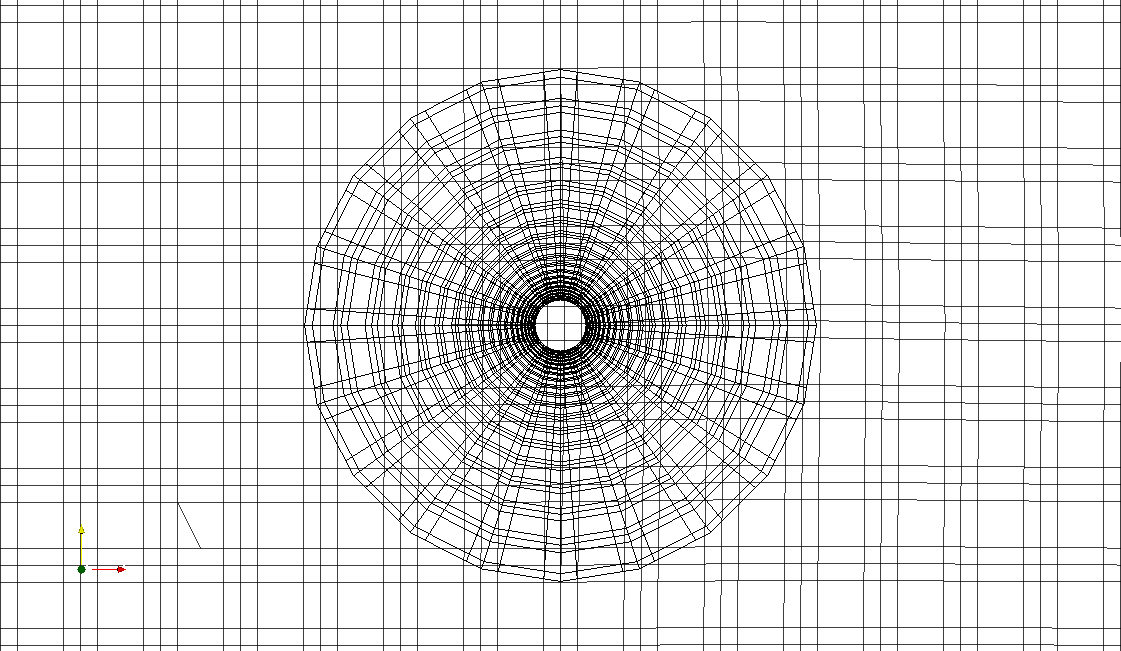
\includegraphics[height=4.3cm]{figs/results/cylinder_overset/lo_overset_cylinder_mesh.png}
		\label{fig:ovs_msh_cyl_lo}
    }
    \subfigure[][High-order cylinder single mesh, P5Q4.]
    {
		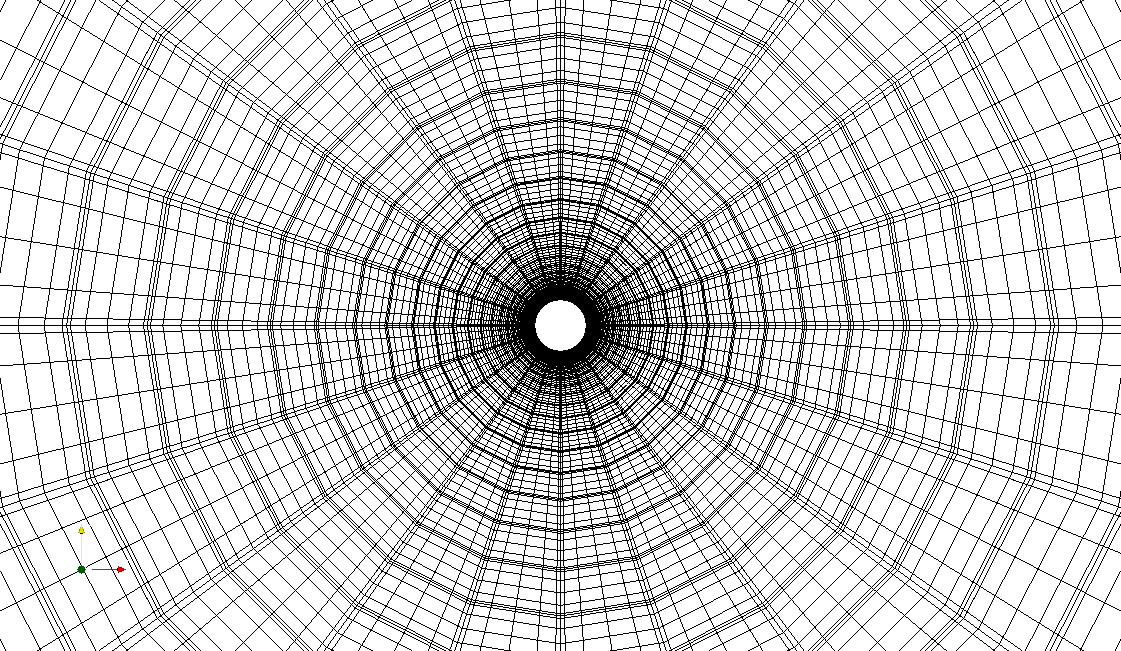
\includegraphics[height=4.3cm]{figs/results/cylinder_overset/ho_cylinder_mesh.png}
		\label{fig:sin_msh_cyl_ho}
    }
    \subfigure[][High-order cylinder overset mesh, P5Q4.]
    {
		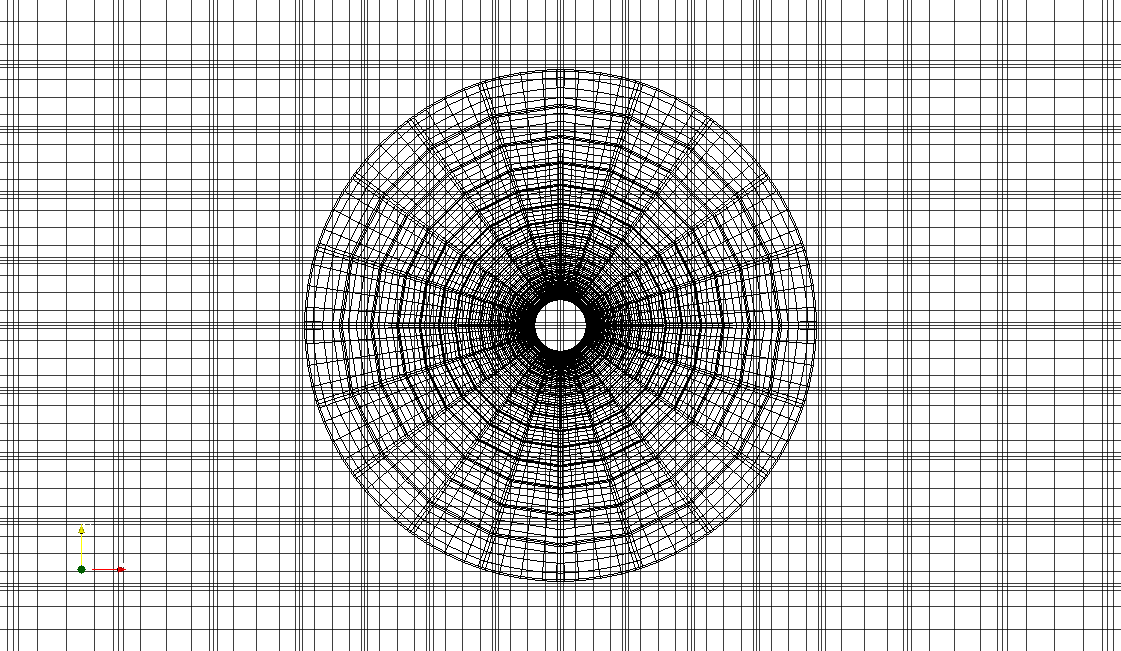
\includegraphics[height=4.3cm]{figs/results/cylinder_overset/ho_overset_cylinder_mesh.png}
		\label{fig:ovs_msh_cyl_ho}
    }
    \caption{Close-up views of the cylinder single and overset Spectral Difference meshes for two different scenarios of mesh and solver orders: P2Q1 and P5Q4.}
    \label{fig:msh_cylinder_sd}
\end{figure}

% describe receptor-donor connectivity
%   - background fringes/holes
%   - near-body fringes
%   - issue with the fringe-circuit related to refinement at the outer near-body boundary (maybe show it visually)
For the overset grid runs, the receptor-donor connectivity outputs special cell tags at a preprocessing stage to identify the fringe and hole cells. Figures\ \ref{fig:bkg_frg_cyl_lo} and \ref{fig:bkg_frg_cyl_ho} illustrate the background  cell tags which are defined as $0$ to represent a fluid (blue), $1$ for hole cells (red), and $2$ for fringe cells (light-gray). Note that the fringe cells in gray formed the fringe-circuit in which the hole cells lay inside with no fluid cell as neighbor. This step is mandatory for the presented methodology due to the assumptions of the hole cell propagating procedure to establish the connectivity. These gray cells are used as donor-receptor interface where the solution transits between the near-body and background meshes. Moreover, in contrast to the background fringe cells, as illustrated in Figs.\ \ref{fig:bdy_frg_cyl_lo} and \ref{fig:bdy_frg_cyl_ho}, the near-body fringe cells are used solely as donors to the ghost flux points at the inner boundary of the background fringe circuit.
% Fringes
\begin{figure}[H]
	\centering
    \subfigure[][Cylinder background special cells (P2Q1).]
    {
		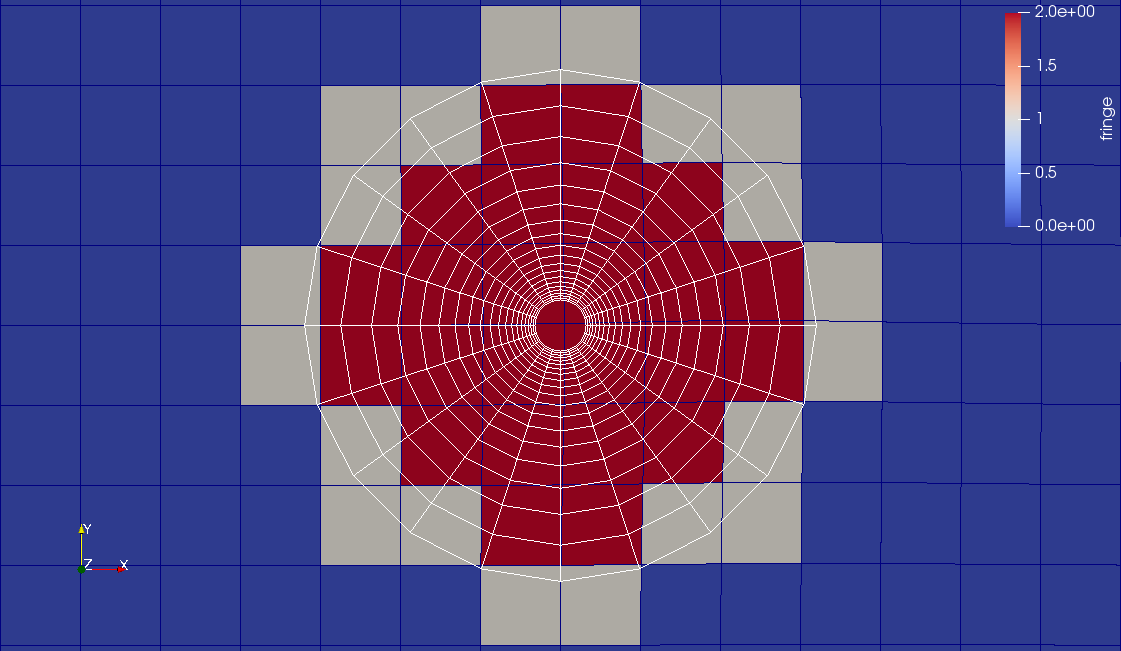
\includegraphics[height=4.3cm]{figs/results/cylinder_overset/lo_overset_cylinder_fringes.png}
		\label{fig:bkg_frg_cyl_lo}
    }
    \subfigure[][Cylinder near-body special cells (P2Q1).]
    {
		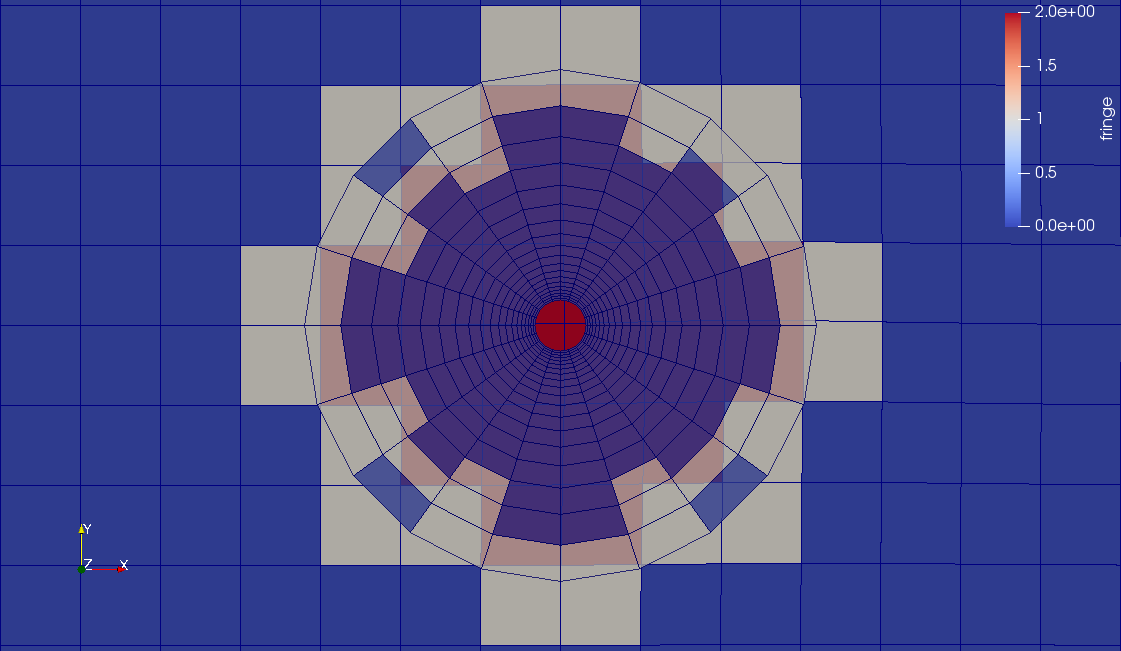
\includegraphics[height=4.3cm]{figs/results/cylinder_overset/lo_overset_cylinder_fringes_body.png}
		\label{fig:bdy_frg_cyl_lo}
    }
    \subfigure[][Cylinder background special cells (P5Q4).]
    {
		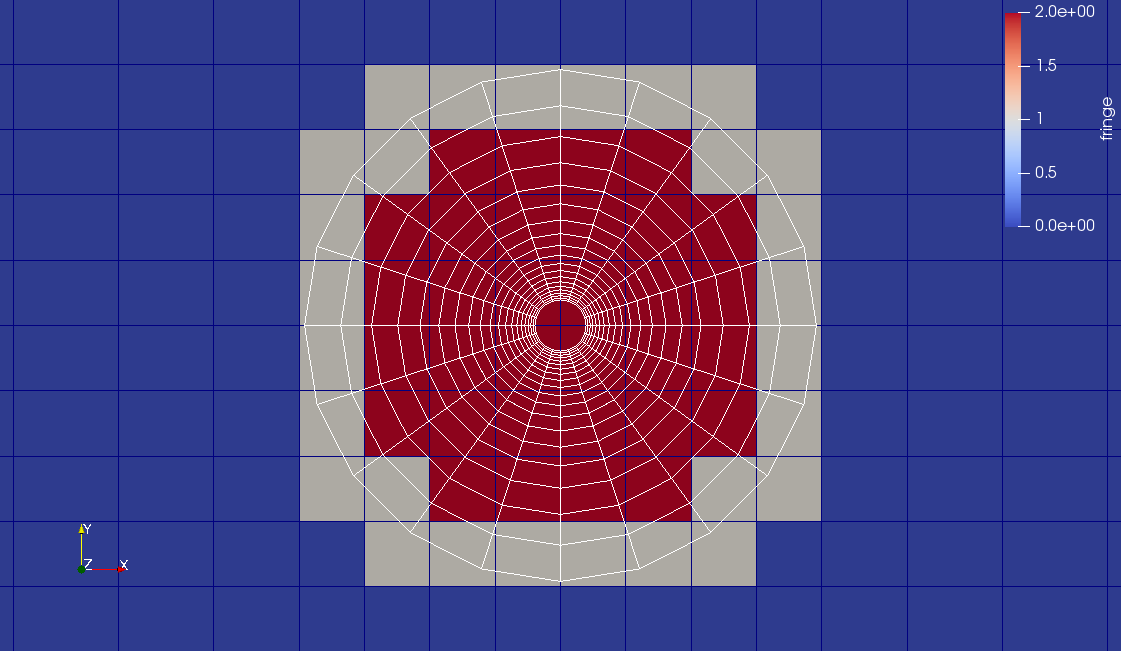
\includegraphics[height=4.3cm]{figs/results/cylinder_overset/ho_overset_fringes.png}
		\label{fig:bkg_frg_cyl_ho}
    }
    \subfigure[][Cylinder near-body special cells (P5Q4).]
    {
		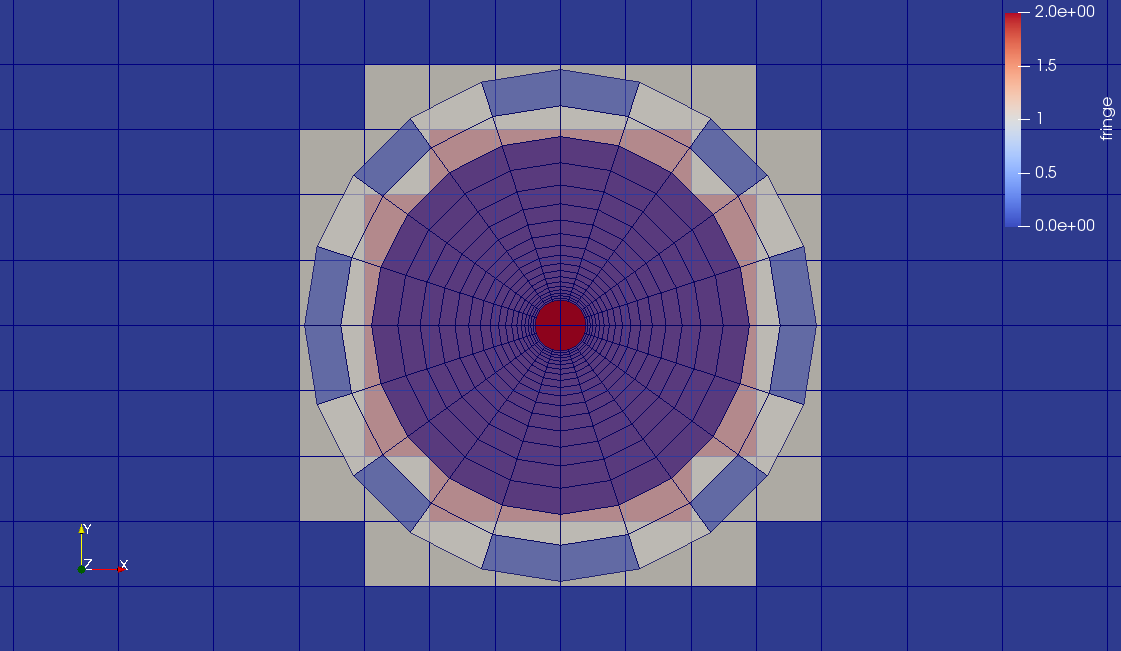
\includegraphics[height=4.3cm]{figs/results/cylinder_overset/ho_overset_fringes_body.png}
		\label{fig:bdy_frg_cyl_ho}
    }
    \caption{Cylinder overset grid special cells for the background (left) and near-body meshes (right). Fringes  in light-gray, holes in red, and fluid cells in blue.}
    \label{fig:frg_cylinder_ho}
\end{figure}

% describe the residue for single and overset 
The results of residue are shown in Fig.\ \ref{fig:cylinder_residue} where the y-axis is the L2-norm order of magnitude of the entire residue vector including all conservative property residue and the x-axis is the number of time iterations. The single mesh results are represented by the mesh size in the legend through the suffix $20 \times 32$, while the overset mesh for low-order is $20 \times 20$\_{$32 \times 32$} and high-order, $20 \times 20$\_{$24 \times 24$}. The rate of change of the residue magnitude for the single mesh results is similar for both single mesh test cases, both reaching around $10^{-7}$ of residue L2-norm in $10^{5}$ iterations. However, a significant difference can be seen when comparing the behavior of the residue for the overset tests. The low-order (P2Q1) overset case reached a $10^{-7.5}$ residue L2-norm in approximately $50,000$ iterations. 

% Residue
\begin{figure}[H]
	\centering
   	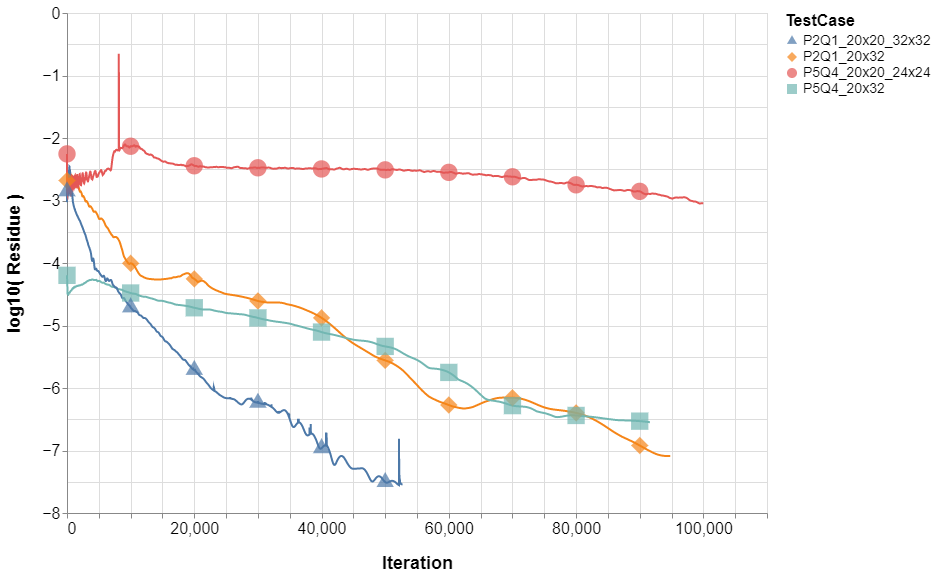
\includegraphics[height=10.0cm]{figs/results/cylinder/residue.png}
    \caption{Comparison of the L2-norm of the density residue for the single and overset cases with different mesh and solver orders.}
    \label{fig:cylinder_residue}
\end{figure}

In contrast, the residue for the high-order (P5Q4) overset case only reached around $10^{-3}$ residue L2-norm at the end of the $10^{5}$ iterations. In fact, by observing the solution throughout the iterations, what has increased its norm its a residue wave that starts at the cylinder wall and propagates up to the outer boundary of the both background and single meshes, where the non-reflective boundary condition allows such wave to exit the computational domain. Nonetheless, due to the small time step, as a result of a higher $P$, and small characteristic length, the number of iterations needed so that this residue wave reaches the outer boundary is very large. The criterion used here to stop the iterations for this scenario was, then, to wait until the residue wave is totally transported from the near-body mesh to a considerable distance out of the fringe circuit of the background mesh. Over this consideration, the residue around the near-body mesh for the high-order overset plunges to $10^{-7}$.
% mach contours
%   - solution colormap ranges from 0.0 to 0.4 with a solution contours with 0.04 step
%   - for overset explain how to read the mach solution (presented solution is on near-body mesh, while the background is represented only by the wireframe colored by the Mach solution)
%   - low mesh order with high reslution does not present double symmetry in both single/overset
%   - high mesh order with high order does in both single/overset

% Mach solution
\begin{figure}[H]
	\centering
    \subfigure[][Single mesh Mach solution.]
    {
		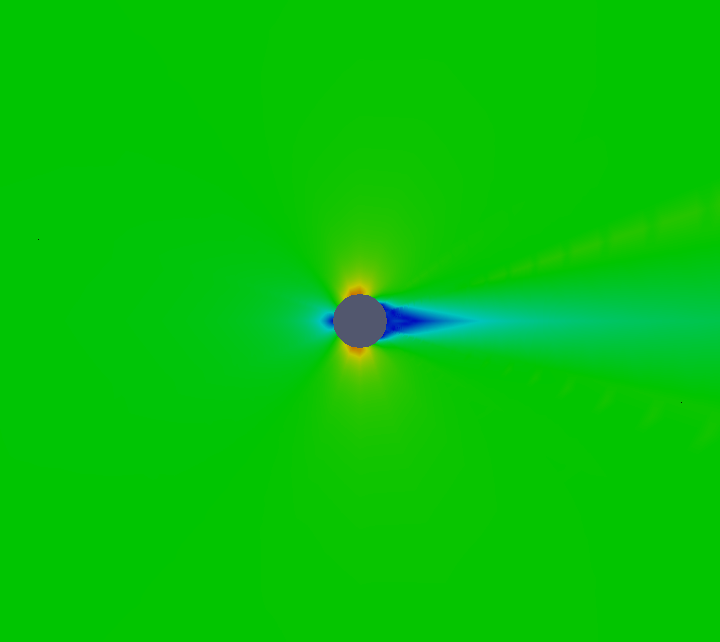
\includegraphics[height=6.3cm]{figs/results/cylinder/solution/mach_single_p2_far.png}
		\label{fig:sin_mach_cyl_lo}
    }
    \subfigure[][Overset mesh Mach solution.]
    {
		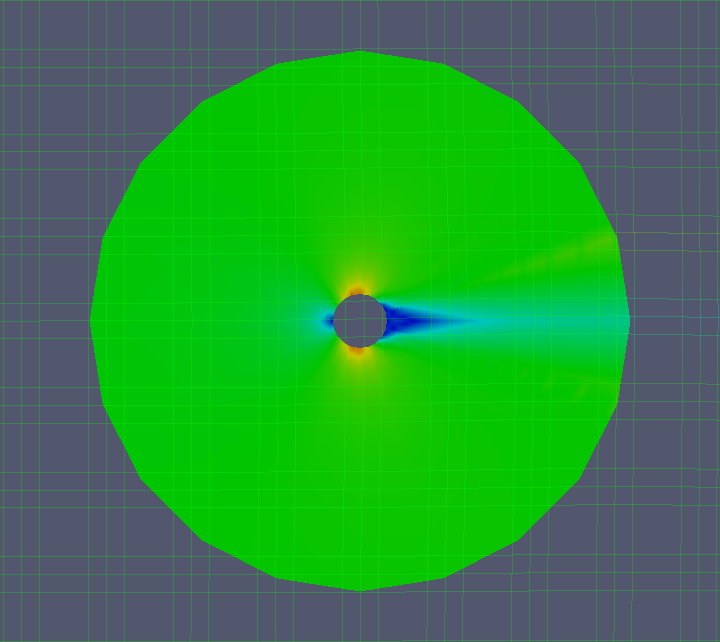
\includegraphics[height=6.3cm]{figs/results/cylinder/solution/mach_overset_p2_far.png}
		\label{fig:ovs_mach_cyl_lo}
    }
     \subfigure[][Single mesh Mach contour close-up.]
    {
		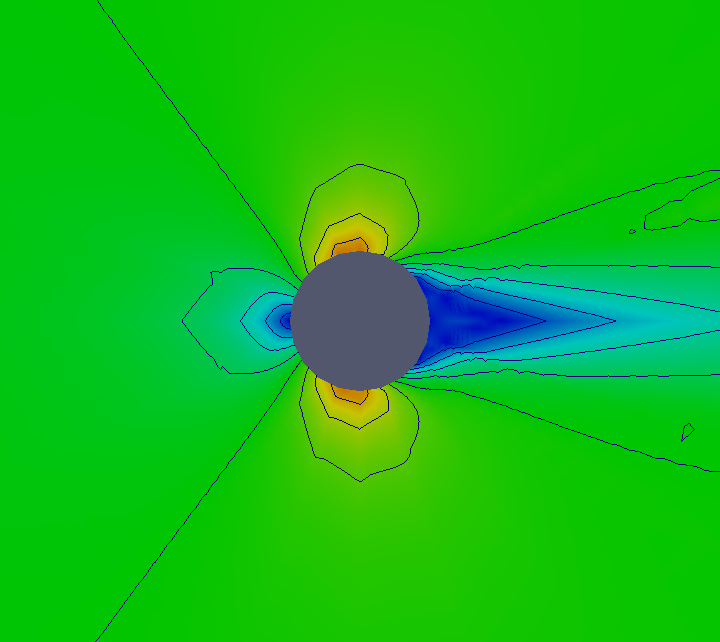
\includegraphics[height=6.3cm]{figs/results/cylinder/solution/mach_c_single_p2.png}
		\label{fig:sin_mach_cyl_lo_c}
    }
    \subfigure[][Overset mesh Mach contour close-up.]
    {
		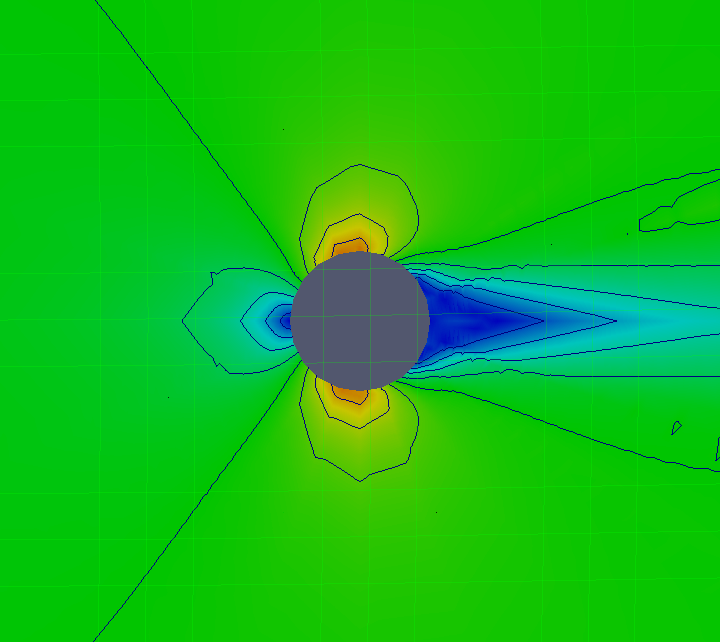
\includegraphics[height=6.3cm]{figs/results/cylinder/solution/mach_c_overset_p2.png}
		\label{fig:ovs_mach_cyl_lo_c}
    }
    \caption{Cylinder single and overset grid solution in terms of Mach number countors for P2Q1.}
    \label{fig:mach_cylinder_lo}
\end{figure}
%   - low mesh order with high reslution does not present double symmetry in both single/overset
%   - high mesh order with high order does in both single/overset

The solution for both single and overset cases converged around $10^{-7}$ of residue magnitude and the Mach number solution is, then, obtained and illustrated in Figs.\ \ref{fig:mach_cylinder_lo} and \ref{fig:mach_cylinder_ho}. The Mach number contours are shown with a fixed colormap ranging from $0.0$ to $0.4$ and step $0.02$ in Figs.\ \ref{fig:sin_mach_cyl_lo_c}, \ref{fig:ovs_mach_cyl_lo_c}, \ref{fig:sin_mach_cyl_ho_c} and \ref{fig:ovs_mach_cyl_ho_c}. For the overset scenarios, the background mesh is presented by the solution wireframe colored by the Mach number while the near-body mesh follows the aforementioned colormap over its solution surface. The reason is to ease the visualization since the data of interest for this test case lies entirely in the near-body mesh. Thus, the background mesh solution here does not provide any additional information. 

The behavior of the solution comparing the single and overset results are nearly identical. In the low-order cases, for both single and overset meshes, even though the solution is 3rd order, i.e., $P=2$, due to the inadequate geometrical representation of the cylinder curvature, a non-physical solution at the cylinder trailing edge is formed which can be observed in Fig.\ \ref{fig:mach_cylinder_lo}. For the high-order cases, instead, the expected solution double symmetry for the inviscid cylinder is presented, as shown in Figs.\ \ref{fig:sin_mach_cyl_ho_c} and \ref{fig:ovs_mach_cyl_ho_c}.

\begin{figure}[H]
	\centering
    \subfigure[][Single mesh Mach solution.]
    {
		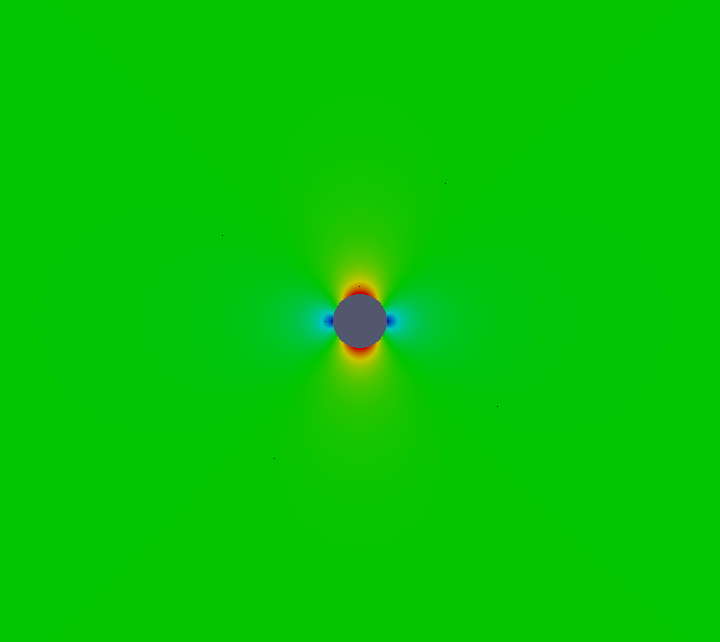
\includegraphics[height=6.3cm]{figs/results/cylinder/solution/mach_single_p5_far.png}
		\label{fig:sin_mach_cyl_ho}
    }
    \subfigure[][Overset mesh Mach solution.]
    {
		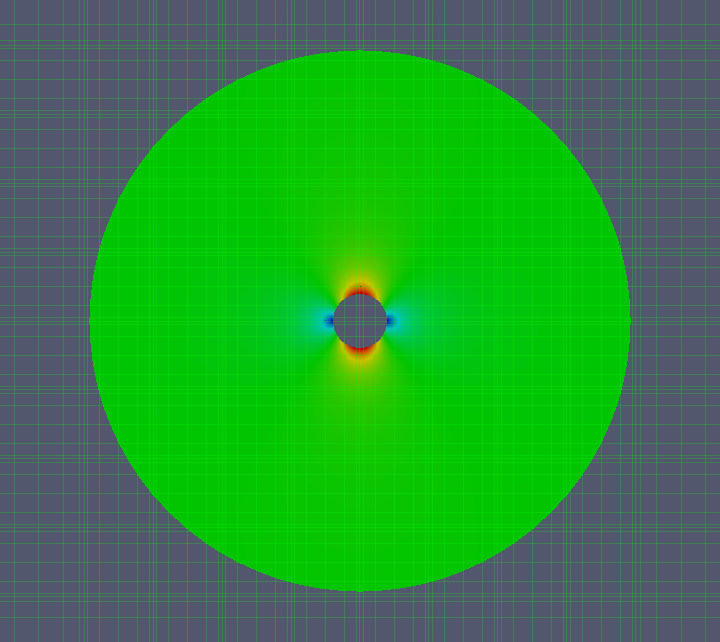
\includegraphics[height=6.3cm]{figs/results/cylinder/solution/mach_overset_p5_far.png}
		\label{fig:ovs_mach_cyl_ho}
    }
     \subfigure[][Single mesh Mach contour close-up.]
    {
		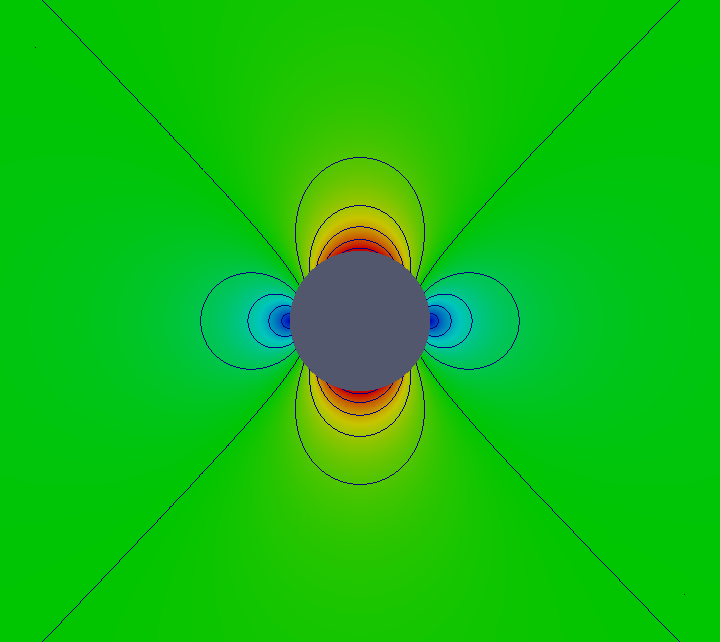
\includegraphics[height=6.3cm]{figs/results/cylinder/solution/mach_c_single_p5.png}
		\label{fig:sin_mach_cyl_ho_c}
    }
    \subfigure[][Overset mesh Mach contour close-up.]
    {
		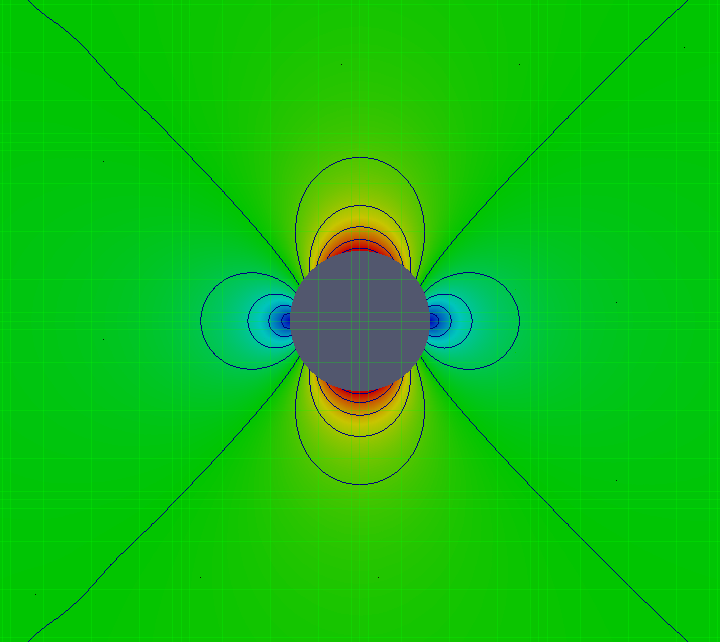
\includegraphics[height=6.3cm]{figs/results/cylinder/solution/mach_c_overset_p5.png}
		\label{fig:ovs_mach_cyl_ho_c}
    }
    \caption{Cylinder single and overset grid solution in terms of Mach number contours for P5Q4.}
    \label{fig:mach_cylinder_ho}
\end{figure}

\section{Isentropic Vortex}

The 2-D inviscid isentropic vortex problem is chosen to benchmark the single and overset numerical solutions. Due to the presence of an analytical solution, it is commonly used in the literature to test the accuracy of an Euler simulation \cite{Yee1999} and, in particular, for high-order methods as a validation test case of the International Workshop on High-Order Methods in CFD \cite{4thHOW} and in several articles \cite{Huynh2014, Crabill2016, DuanThesis2019}.

The mean flow properties considered to be the freestream $u_{\infty}$ and $v_{\infty}$ as the velocity components, $\rho_{\infty}$ as density, $p_{\infty}$ as pressure,  $T_{\infty}$ as temperature, with the values ($u_{\infty}$=1, $v_{\infty}$=1, $\rho_{\infty}$=1, $p_{\infty}$=1, $T_{\infty}$=1). The mean flow velocity components here define how the vortex is transported. The vortex center position, ($x_c$, $y_c$), can be determined at any time $t$ by $x_0 + u_{\infty}t$ and $y_0 + v_{\infty}t$ and ($x_0$=0, $y_0$=0) is the initial coordinates of the vortex center. The initial condition for the single and overset tests is the analytical solution for the inviscid isentropic vortex with no perturbation in entropy ($\delta S=0$) for the mean flow field. The perturbations in velocity and temperature can be given by
% Problem setup
%
\begin{equation}
    \label{eq_vortex_analytical_1}
	\delta u = 	-\frac{\Delta y \beta}{2\pi} e^{\frac{1-r^2}{2}},\\
	\delta v = 	\frac{\Delta x \beta}{2\pi} e^{\frac{1-r^2}{2}},
\end{equation}
%
\begin{equation}
    \label{eq_vortex_analytical_2}
	\delta T = 	-\frac{(\gamma-1)\beta}{8\gamma\pi} e^{1-r^2}
\end{equation}
where $\delta u$ and $\delta v$ are, respectively, the perturbations of the velocity in x and y direction and $\delta T$ is the perturbation in the fluid temperature. The $\beta$ parameter is the vortex strength, the coordinates ($\Delta x$, $\Delta y$) = ($x-x_0$, $x-x_0$), and $r^2 = ({\Delta x}^2+{\Delta y}^2)$. The fluid is assumed as a perfect gas with $\gamma$=1.4 for air. From the isentropic relations, the conservative fluid properties $\rho = \rho_{\infty} + \delta \rho$, $u = u_{\infty} + \delta u$, $v = v_{\infty} + \delta v$, $T = T_{\infty} + \delta T$ can be determined by

\begin{equation}
    \label{eq_vortex_analytical_3}
	\rho = T^{\frac{1}{\gamma-1}} = {(T_{\infty} + \delta T)}^{\frac{1}{\gamma-1}},
\end{equation}
%
\begin{equation}
    \label{eq_vortex_analytical_4}
	\rho u = \rho (u_{\infty} + \delta u),
\end{equation}
%
\begin{equation}
    \label{eq_vortex_analytical_5}
	\rho v = \rho (v_{\infty} + \delta v),
\end{equation}
%
\begin{equation}
    \label{eq_vortex_analytical_6}
	p = \rho^{\gamma},
\end{equation}
%
\begin{equation}
    \label{eq_vortex_analytical_7}
	E = \frac{p}{\gamma-1} + \frac{1}{2}\rho [{(u_{\infty} + \delta u)}^2 + {(v_{\infty} + \delta v)}^2].
\end{equation}

% BC model setup
The boundary conditions used for the overset test case over the isentropic vortex problem are a non-reflective farfield at the outer boundary of the background mesh and an overset boundary condition at the near-body mesh outer boundary. This is imposed at the mesh generation stage. In the present work, the open source GMSH software is used for this matter \cite{Geuzaine2009Gmsh}. Several scenarios are tested for this problem combining three different meshes with $16 \times 16$, $32 \times 32$, and $64 \times 64$ cells for the background mesh and, respectively, $5 \times 5$, $10 \times 10$, and $20 \times 20$ near-body mesh. For single mesh cases, the background meshes are used. For instance, Figs.\ \ref{fig:overset_vortex_mesh_bkg} and \ref{fig:overset_vortex_mesh_bdy} show a $32 \times 32$ cell background mesh and a $10 \times 10$ cell near-body mesh. The latter is rotated 45 degrees so that its right outer boundary face is aligned with the vortex velocity. The tests provided for this problem included several different orders of accuracy of the Spectral Difference method, ranging from $P=2$ to $P=6$. Figure\ \ref{fig:overset_vortex_sd_mesh} illustrates the $32 \times 32$ background and $10 \times 10$ near-body meshes for the Spectral Difference method with orders ranging from $P=2$ to $P=4$.
% Meshes (single and overset)
% Initial Mesh
\begin{figure}[H]
	\centering
    \subfigure[][Close-up snapshot of the overset mesh.]
    {
		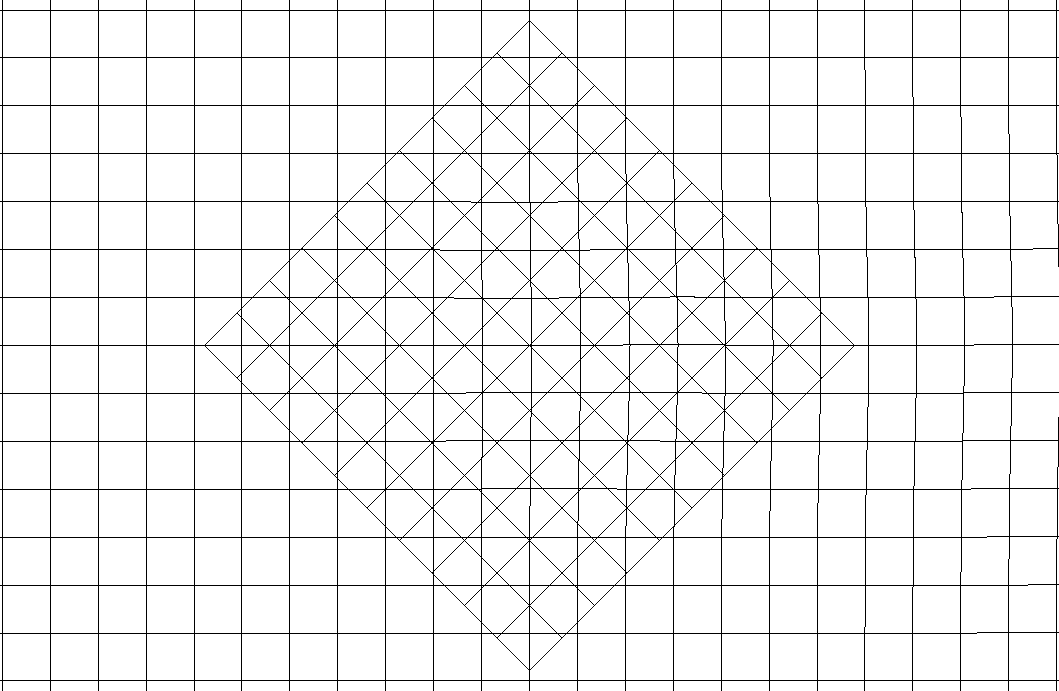
\includegraphics[height=4.0cm]{figs/results/vortex_32_10/close_up.png}
		\label{fig:overset_vortex_mesh_bkg}
    }
     \subfigure[][Overset mesh.]
    {
		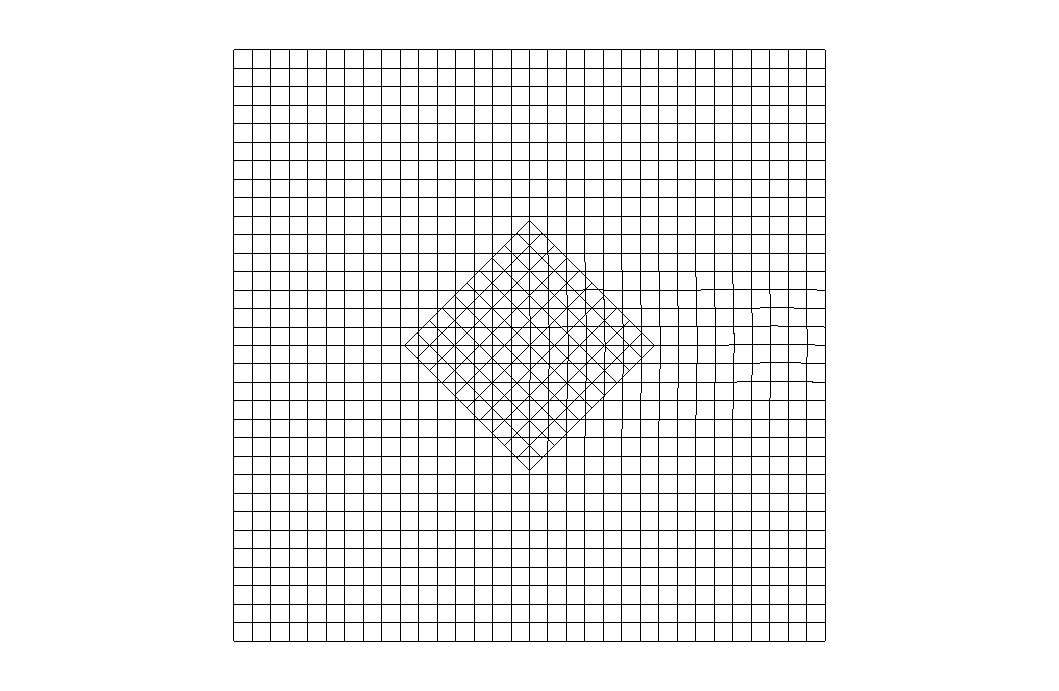
\includegraphics[height=4.0cm]{figs/results/vortex_32_10/overset_mesh.png}
		\label{fig:overset_vortex_mesh_bdy}
    }
    \subfigure[][P=2 close-up view.]
    {
		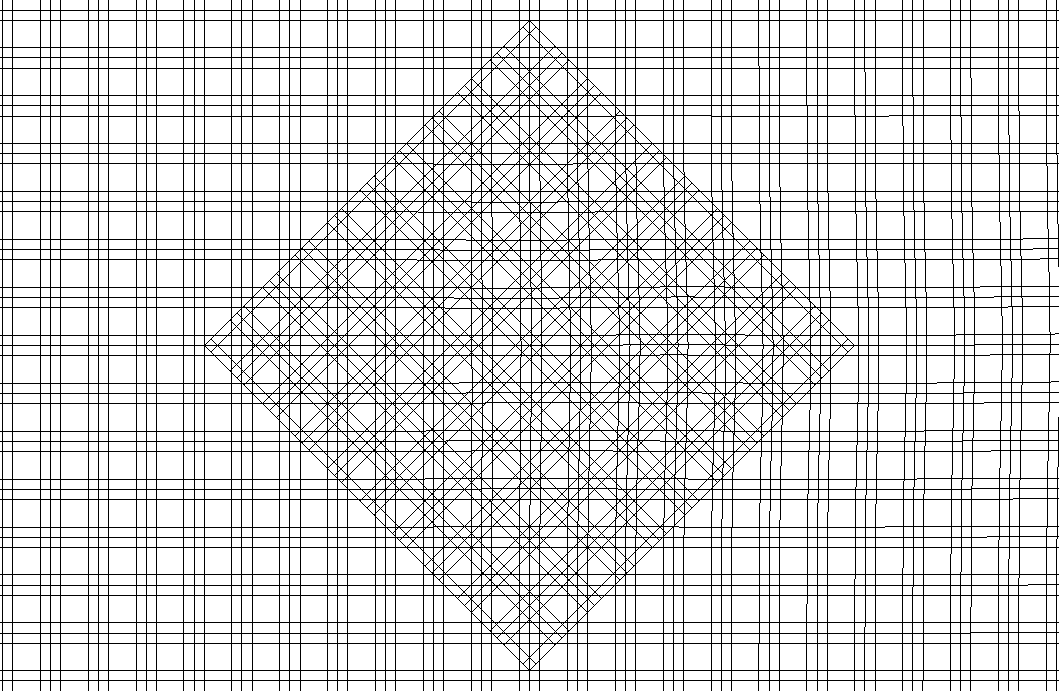
\includegraphics[height=4.0cm]{figs/results/vortex_32_10/p=2/close_up.png}
		\label{fig:overset_vortex_p2_mesh_bkg}
    }
     \subfigure[][P=2 overall view.]
    {
		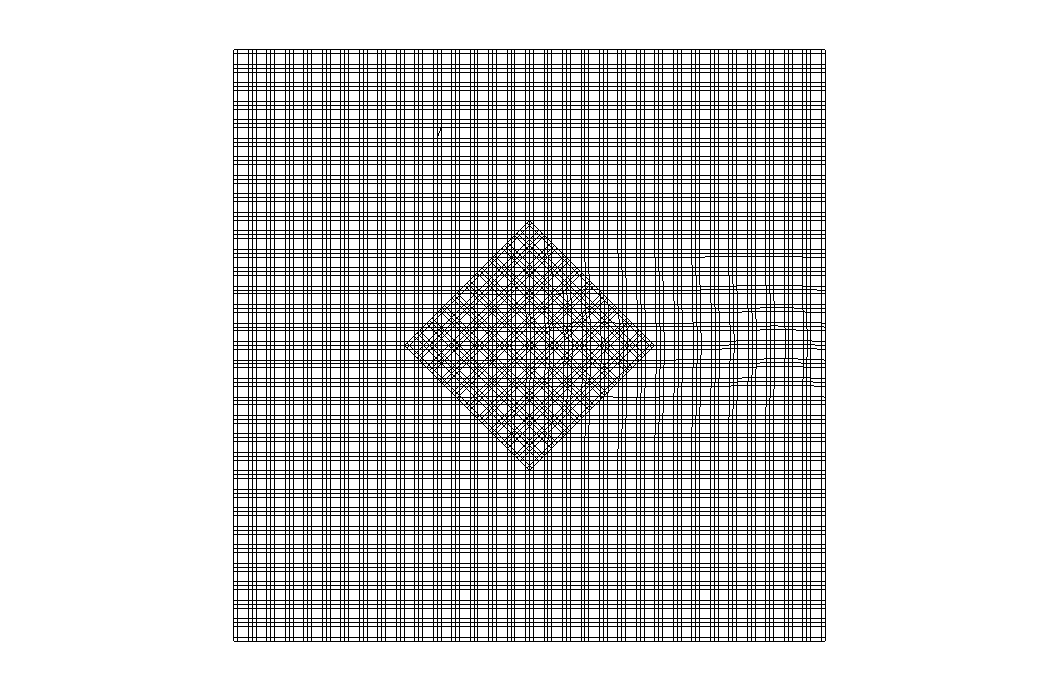
\includegraphics[height=4.0cm]{figs/results/vortex_32_10/p=2/mesh_p.png}
		\label{fig:overset_vortex_p2_mesh_bdy}
    }
    \subfigure[][P=3 close-up view.]
    {
		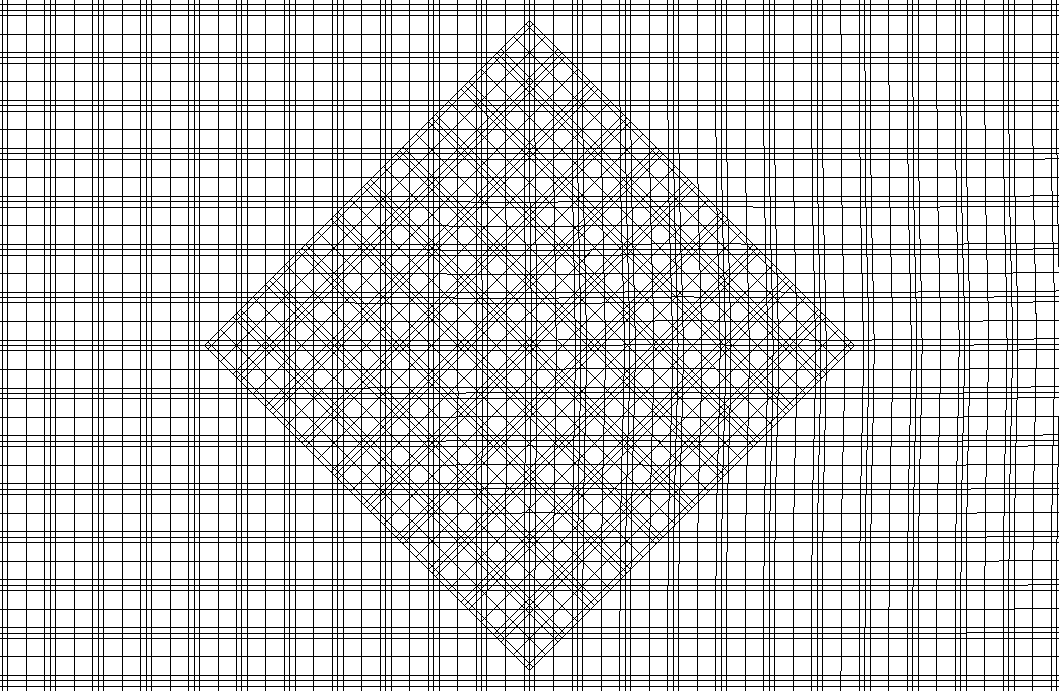
\includegraphics[height=4.0cm]{figs/results/vortex_32_10/p=3/close_up.png}
		\label{fig:overset_vortex_p3_mesh_bkg}
    }
     \subfigure[][P=3 overall view.]
    {
		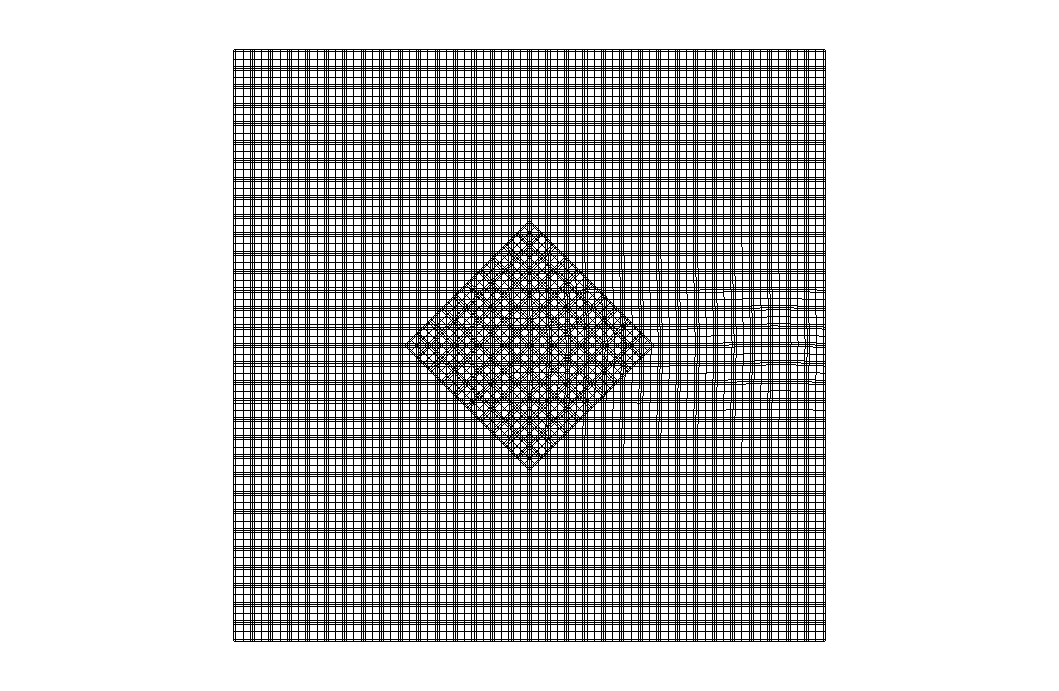
\includegraphics[height=4.0cm]{figs/results/vortex_32_10/p=3/mesh_p.png}
		\label{fig:overset_vortex_p3_mesh_bdy}
    }
    \subfigure[][P=4 close-up view]
    {
		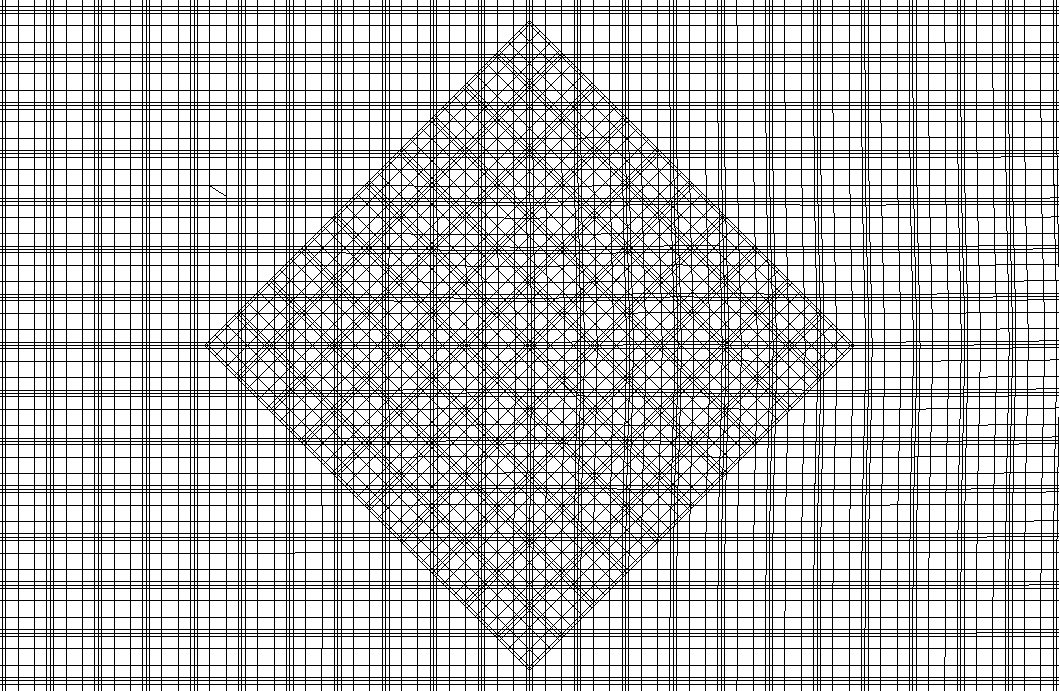
\includegraphics[height=4.0cm]{figs/results/vortex_32_10/p=4/close_up.png}
		\label{fig:overset_vortex_p4_mesh_bkg}
    }
     \subfigure[][P=4 overall view.]
    {
		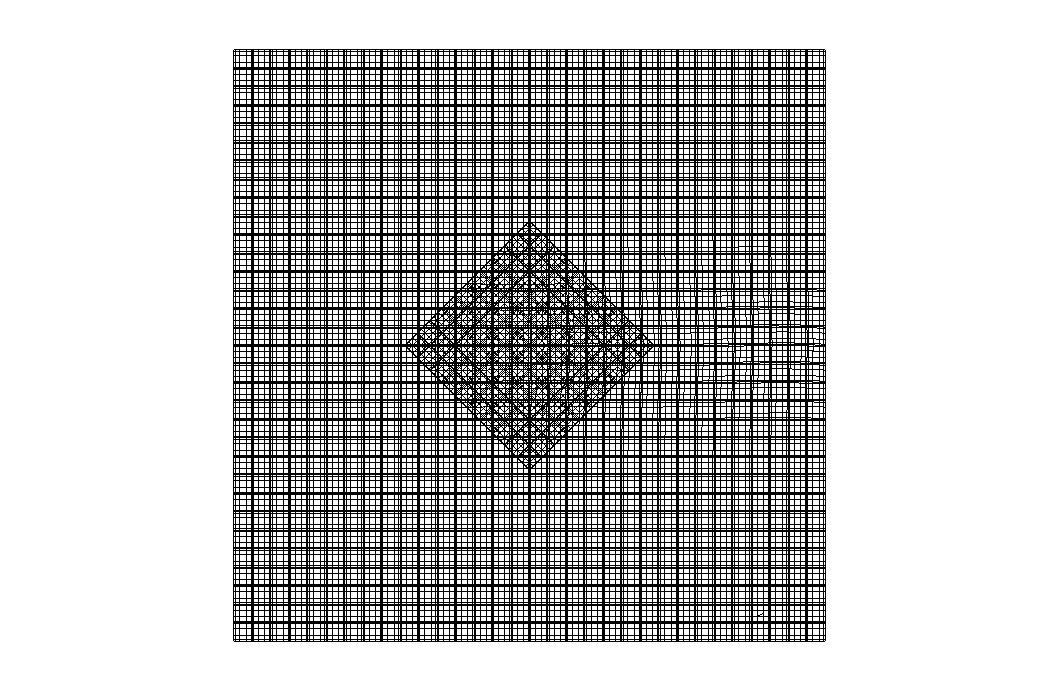
\includegraphics[height=4.0cm]{figs/results/vortex_32_10/p=4/mesh_p.png}
		\label{fig:overset_vortex_p4_mesh_bdy}
    }
    \caption{Spectral Difference mesh for the $32 \times 32$ background and $10 \times 10$ near-body mesh case.}
    \label{fig:overset_vortex_sd_mesh}
\end{figure}
%
%
The initial solution is given by the analytical solution described in Eqs.\ \ref{eq_vortex_analytical_3}, \ref{eq_vortex_analytical_4}, \ref{eq_vortex_analytical_5}, \ref{eq_vortex_analytical_7} and the initial solution for the density contours can be seen in Fig.\ \ref{fig:overset_vortex_initial solution}. Note that the setup of the near-body mesh is precisely built so that the entire vortex fits inside the near-body mesh in the initial solution. Figure\ \ref{fig:bkg_vortex_init_sol} shows the initial density solution at background mesh where the hole cells can be seen fully overlapped by the near-body mesh. Figure\ \ref{fig:bdy_vortex_init_sol} shows the near-body mesh initial density solution. Figure\ \ref{fig:ovs_vortex_init_sol} shows the overall overset initial density solution for both background and near-body mesh.
%

\begin{figure}[H]
	\centering
	\subfigure[][]
    {
    	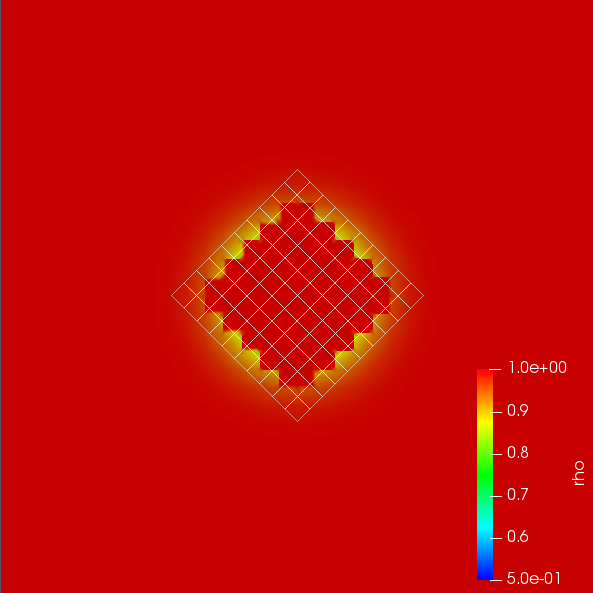
\includegraphics[height=5.0cm]{figs/results/vortex_32_10/background_initial_solution.png}
    	\label{fig:bkg_vortex_init_sol}
    }
    \subfigure[][]
    {
    	\includegraphics[height=5.0cm]{figs/results/vortex_32_10/nearbody_initial_solution_2.png}
    	\label{fig:bdy_vortex_init_sol}
    }
    \subfigure[][]
    {
    	\includegraphics[height=5.0cm]{figs/results/vortex_32_10/initial_solution_density.png}
    	\label{fig:ovs_vortex_init_sol}
    }
	\caption{Initial solution for the density in the overset setup.}
    \label{fig:overset_vortex_initial solution}
\end{figure}

% describe receptor-donor connectivity
%   - background fringes/holes
%   - near-body fringes
%   - issue with the fringe-circuit related to refinement at the outer near-body boundary (maybe show it visually)
Figure\ \ref{fig:overset_vortex_fringes} presents the background and near-body mesh special cell tags. The fringe cells are represented here in light-blue color, hole cells in light-orange and the reactivated hole cells in red. Note that for the near-body fringes, since only the inward background fringe circuit receives data from the near-body mesh, the addition of flux-points in the background cells due to higher $P$ values increases the number of near-body fringes. In all scenarios, the fringe circuit is formed as can be seen in Figs.\ \ref{fig:overset_vortex_p2_fringes_bkg}, \ref{fig:overset_vortex_p3_fringes_bkg}, and \ref{fig:overset_vortex_p4_fringes_bkg}.

% Fringes
\begin{figure}[H]
	\centering
    \subfigure[][Background fringe and hole cells, P=2.]
    {
		\includegraphics[height=5.0cm]{figs/results/vortex_32_10/p=2/bkg_fringes.png}
		\label{fig:overset_vortex_p2_fringes_bkg}
    }
     \subfigure[][Near-body fringe cells, P=2.]
    {
		\includegraphics[height=5.0cm]{figs/results/vortex_32_10/p=2/near_body_fringes.png}
		\label{fig:overset_vortex_p2_fringes_bdy}
    }
    \subfigure[][Background fringe and hole cells, P=3.]
    {
		\includegraphics[height=5.0cm]{figs/results/vortex_32_10/p=3/bkg_fringes.png}
		\label{fig:overset_vortex_p3_fringes_bkg}
    }
     \subfigure[][Near-body fringe cells, P=3.]
    {
		\includegraphics[height=5.0cm]{figs/results/vortex_32_10/p=3/near_body_fringes.png}
		\label{fig:overset_vortex_p3_fringes_bdy}
    }
    \subfigure[][Background fringe and hole cells, P=4.]
    {
		\includegraphics[height=5.0cm]{figs/results/vortex_32_10/p=4/bkg_fringes.png}
		\label{fig:overset_vortex_p4_fringes_bkg}
    }
     \subfigure[][Near-body fringe cells, P=4.]
    {
		\includegraphics[height=5.0cm]{figs/results/vortex_32_10/p=4/near_body_fringes.png}
		\label{fig:overset_vortex_p4_fringes_bdy}
    }
    \caption{Fringe and hole cells for different orders of accuracy of the Spectral Difference method in the overset vortex case.}
    \label{fig:overset_vortex_fringes}
\end{figure}

% Flux point out of the near-body outer boundary
A special edge case is addressed in this test when a flux-point located at the fringe-circuit interface is not overlapped by the near-body mesh. As illustrated in Fig.\ \ref{fig:overset_vortex_special_fringes}, the green orange dots represent interface flux points of some background fringe cells. The white wireframe is the near-body mesh, and  as it can be seen, the green dots lay outside of the near-body outer boundary. Therefore, no receptor-donor connectivity can be established since the interpolation is only defined within a cell domain. The proposed solution for this issue is to reactivate the hole cells represented in red that own flux points with no near-body cell overlapping. The reactivation restores the unstructured cell connectivity between the reactivated cell and its fringe cell neighbors and tag this hole cell as a fringe cell. Then, the reactivated cell becomes part of the fringe circuit and its flux points interfaces are searchable to establish additional receptor-donor connectivity.

\begin{figure}[H]
	\centering
	\includegraphics[height=10.0cm]{figs/results/vortex_32_10/p=3/closeup_flux_point_markers.jpg}
    \caption{Special case when a flux-point of a fringe cell is out of the near-body mesh (green dots). Background fringe cells in light blue, hole cells in light orange and the special case of fringe cells in red.}
    \label{fig:overset_vortex_special_fringes}
\end{figure}

% density solution
%   - solution colormap ranges from 0.0 to 0.4 with a solution contours with 0.04 step
%   - for overset explain how to read the mach solution (presented solution is on near-body mesh, while the background is represented only by the wireframe colored by the Mach solution)
%   - low mesh order with high reslution does not present double symmetry in both single/overset
%   - high mesh order with high order does in both single/overset
The solution in terms of density contours for the selected mesh of $32 \times 32$ background and $10 \times 10$ near-body meshes can be seen in Fig.\ \ref{fig:overset_vortex_rho}. The density contours are presented through a colormap ranging from $0.5$ to $1.0$ and three time periods are chosen to present the solution: $t=0$ (initial solution), $t=20$, and $t=50$. The time here is normalized so that the $t=100$ would indicate the time at which the vortex center is located at the upper-right edge in the background mesh. Additionally, Figure\ \ref{fig:overset_vortex_rho} shows the results for different orders of accuracy of the Spectral Difference method from $P=2$ to $P=4$. The numerical solution at $t=20$ represents the simulation time where half of the vortex is in the near-body mesh and the other half in the background mesh, as demonstrated in Figs.\ \ref{fig:overset_vortex_p2_rho_t20}, \ref{fig:overset_vortex_p3_rho_t20}, and \ref{fig:overset_vortex_p4_rho_t20}. For $t=50$ the vortex is completely transported to the background mesh with its magnitude and symmetry preserved for both setups.
% DENSITY SOLUTION FOR OVERSET VORTEX
\begin{figure}[H]
	\centering
    \subfigure[][P=2 and t=0 (initial solution).]
    {
		\includegraphics[height=3.2cm]{figs/results/vortex_32_10/p=2/rho_t_0.png}
		\label{fig:overset_vortex_p2_rho_t0}
    }
     \subfigure[][P=2 and t=20.]
    {
		\includegraphics[height=3.2cm]{figs/results/vortex_32_10/p=2/rho_t_25.png}
		\label{fig:overset_vortex_p2_rho_t20}
    }
    \subfigure[][P=2 and t=50.]
    {
		\includegraphics[height=3.2cm]{figs/results/vortex_32_10/p=2/rho_t_50.png}
		\label{fig:overset_vortex_p2_rho_t50}
    }
    \subfigure[][P=3 and t=0 (initial solution).]
    {
		\includegraphics[height=3.2cm]{figs/results/vortex_32_10/p=3/rho_t_0.png}
		\label{fig:overset_vortex_p3_rho_t0}
    }
     \subfigure[][P=3 and t=20.]
    {
		\includegraphics[height=3.2cm]{figs/results/vortex_32_10/p=3/rho_t_25.png}
		\label{fig:overset_vortex_p3_rho_t20}
    }
    \subfigure[][P=3 and t=50.]
    {
		\includegraphics[height=3.2cm]{figs/results/vortex_32_10/p=3/rho_t_50.png}
		\label{fig:overset_vortex_p3_rho_t50}
    }
    \subfigure[][P=4 and t=0 (initial solution).]
    {
		\includegraphics[height=3.2cm]{figs/results/vortex_32_10/p=4/rho_t_0.png}
		\label{fig:overset_vortex_p4_rho_t0}
    }
     \subfigure[][P=4 and t=20.]
    {
		\includegraphics[height=3.2cm]{figs/results/vortex_32_10/p=4/rho_t_25.png}
		\label{fig:overset_vortex_p4_rho_t20}
    }
    \subfigure[][P=4 and t=50.]
    {
		\includegraphics[height=3.2cm]{figs/results/vortex_32_10/p=4/rho_t_50.png}
		\label{fig:overset_vortex_p4_rho_t50}
    }
    \caption{Numerical density contours for the solution of the vortex overset case with P=4 after different time periods.}
    \label{fig:overset_vortex_rho}
\end{figure}

In order to measure the accuracy of the presented overset methodology, since the isentropic vortex problem presents an analytical solution and an isentropic property, the L2-norm of the entropy error is used. Several scenarios are simulated including different orders of accuracy of the Spectral Difference method and different mesh refinements for both single and overset mesh. The single mesh tests are done by using the background mesh only. Figure\ \ref{fig:entropy_vortex} demonstrates the results obtained for these runs. The y-axis is the L2-norm of the entropy error and the x-axis represents the Spectral Difference method polynomial order, {\em i.e.}, $P$. The dashed lines are the results for the single mesh cases, while the solid lines represent the overset mesh cases. For a given mesh refinement, by increasing the solver order, the entropy error magnitude decays in a nearly linear rate, in the log scale, reaching low entropy errors.
%
\begin{figure}[H]
	\centering
   	\includegraphics[height=13.0cm]{figs/results/vortex_32_10/entropy_error.png}
    \caption{Comparison of the L2-norm of the entropy error for the single and overset cases with different values for $P$ and mesh size.}
    \label{fig:entropy_vortex}
\end{figure}

%
\begin{table}[h]
	\centering
    \caption{Values of the median CPU time per iteration in milliseconds.}
    \label{table:cpu_time_table}
    \begin{tabular}{@{}c|ccc|ccc@{}}
    \hline
    \hline
    & \multicolumn{3}{c|}{\textbf{Single}} & \multicolumn{3}{c}{\textbf{Overset}} \\ \hline
    \textbf{p} & 16x16      & 32x32      & 64x64      & 16x16\_5x5 & 32x32\_10x10 & 64x64\_20x20 \\ \hline
    2          & 17         & 76         & 304        & 15          & 63           & 264          \\ 
    3          & 34         & 153        & 602        & 31          & 127          & 510          \\ 
    4          & 66         & 278        & 1132       & 59          & 241          & 945          \\ 
    5          & 129        & 503        & -          & 113         & 436          & -            \\ 
    6          & 217        & -          & -          & 200         & -            & -            \\ 
    \hline
    \hline
    \end{tabular}
\end{table}

Table\ \ref{table:cpu_time_table} shows results of the median CPU time per numerical iteration for the same range of $P$ and mesh size. The CPU time results show that the current implementation of the overset code have presented a lower median CPU time per iteration in all experiments in comparison with the single mesh cases. Since the overset residue calculation is solved asynchronously for both meshes in the overset setup, the additional time cost due to the overset data communication are being compensated by the parallel residue calculation of the overset meshes. Note that the parallelism here is only over the meshes, not the cells. The residue is still calculated sequentially per cell in both single and overset cases.
